
%%%%%%%%%%%%%%%%%%%%%%%%%%%%%%%%%%%%%%%%%%%%%%%%%%%%%%%%%%%%%%%%%%%%%%%%%%%%%
%%% LaTeX-Rahmen fuer das Erstellen von Masterarbeiten
%%%%%%%%%%%%%%%%%%%%%%%%%%%%%%%%%%%%%%%%%%%%%%%%%%%%%%%%%%%%%%%%%%%%%%%%%%%%%

%%%%%%%%%%%%%%%%%%%%%%%%%%%%%%%%%%%%%%%%%%%%%%%%%%%%%%%%%%%%%%%%%%%%%%%%%%%%%
%%% allgemeine Einstellungen
%%%%%%%%%%%%%%%%%%%%%%%%%%%%%%%%%%%%%%%%%%%%%%%%%%%%%%%%%%%%%%%%%%%%%%%%%%%%%
% !TeX spellcheck = en_GB
\documentclass[twoside,12pt,a4paper]{report}
%\usepackage{reportpage}
\usepackage[utf8]{inputenc} % yay encoding
\PassOptionsToPackage{hyphens}{url} % URLs bei Bindestrichen trennen
\usepackage{hyperref} % klickbare Fusnnoten und Verweise
\usepackage{url} % URLs
\usepackage{setspace} % flexiblere Abstaende
\usepackage[british]{babel} % Sprachpaket
\usepackage{graphics, graphicx} % Inclucegraphics
\usepackage{color} % Farben fuer Listings
\usepackage{latexsym}
\usepackage[center]{caption} % Caption-Text zentrieren
\usepackage{eurosym} % Euro-Symbol (ja, wirklich)
\usepackage{etoolbox}
\usepackage{subfig} % Figures mit Unterfigures
\usepackage{geometry} % Raender on-demand anpassen
\usepackage{titlesec} % Titelformat von Kapiteln
\usepackage{tipa} % IPA-Lautschrift
\usepackage{todonotes} % \todo-Befehl
\usepackage{amsmath} % Mathekrams
\usepackage{amssymb} % Mathesymbole
\usepackage[shortcuts]{extdash}
\usepackage[listings,skins]{tcolorbox} % Landscape-Listings in Portrait-Seiten
\usepackage{rotating} % Inhalte drehen
% Tabellenkrams
\usepackage{multirow}
\usepackage{tabularx}
\usepackage{arydshln}

\setlength\dashlinedash{0.2pt}
\setlength\dashlinegap{1.5pt}
\setlength\arrayrulewidth{0.3pt}

\usepackage[normalem]{ulem}
\useunder{\uline}{\ul}{}
\usepackage[printonlyused,withpage]{acronym} % Abkuerzungen richtig einfuehren
\usepackage[margin=10pt,font=small,labelfont=bf]{caption}
\author{Jules Kreuer}
\usepackage[titletoc,toc,page, title]{appendix} % Anhang
\renewcommand*\appendixpagename{Appendix} % Titel einer Anhang-Seite
\renewcommand*\appendixtocname{Appendix} % Anhang-Formatierung im Inhaltsverzeichnis

\definecolor{pblue}{rgb}{0.13,0.13,1}
\definecolor{pgreen}{rgb}{0,0.5,0}
\definecolor{pred}{rgb}{0.9,0,0}
\definecolor{pgrey}{rgb}{0.46,0.45,0.48}
\definecolor{codegrey}{rgb}{0.95,0.95,0.95}


% !TeX TXS-program:compile = txs:///pdflatex/[--shell-escape]
\pdfsuppresswarningpagegroup=1

\usepackage{minted}
\renewcommand{\lstlistingname}{Code} % Caption einzelner Codesnippets
\renewcommand{\lstlistlistingname}{Codeverzeichnis} % Ueberschrift der List of Listings

% Argmin<
\DeclareMathOperator*{\argmin}{argmin}

%Bulletpoints itemize
\renewcommand{\labelitemii}{\textbullet}


% Abstand vor/nach Blockquotes
\expandafter\def\expandafter\quote\expandafter{\quote\onehalfspacing}

% Titelformat in "Kapitel X: Titel" ändern
\titleformat{\chapter}
{\normalfont\LARGE\bfseries}{Chapter \thechapter:}{0.3em}{}
\titlespacing*{\chapter}{0pt}{3.5ex plus 1ex minus .2ex}{2.3ex plus .2ex}

\textwidth 15cm
\textheight 23cm
\topmargin 0.0cm
\evensidemargin 1cm
\oddsidemargin 1cm
\footskip 2cm
\parskip0.5explus0.1exminus0.1ex

% Whitespace! Whitespace everywhere!
\geometry{a4paper,top=25mm, bottom=3cm}
\parindent 0px

%larger tabels
\usepackage{changepage}

% adjust table to page width
\usepackage{adjustbox}

% Kann von Student auch nach pers\"onlichem Geschmack ver\"andert werden.
\pagestyle{headings}

% BibLaTex anstatt BibTeX verwenden
\usepackage[style=alphabetic,backend=biber]{biblatex}
\usepackage[babel]{csquotes}
%\setcitestyle{authoryear, round, citesep={;}, aysep={,}, yysep={;}}
\bibliography{thesis.bib}
%\nocite{*}

\newcommand{\td}[1]{\todo[color=green!40]{#1}}

\begin{document}

%%%%%%%%%%%%%%%%%%%%%%%%%%%%%%%%%%%%%%%%%%%%%%%%%%%%%%%%%%%%%%%%%%%%%%%%%%%%
%%% Titelseite
%%%%%%%%%%%%%%%%%%%%%%%%%%%%%%%%%%%%%%%%%%%%%%%%%%%%%%%%%%%%%%%%%%%%%%%%%%%%

\begin{titlepage}
    \newgeometry{top=25mm, left=30mm, right=30mm, bottom=30mm}
    \begin{center}
        {\LARGE University of T\"ubingen}\\
        {\large Faculty of Science \\
        Department of Computer Science\\[4cm]}
        {\huge Master Thesis Bioinformatics\\[2cm]}
        {\Large\bf Simulating and estimating the effect of gene transfer on bacterial pangenomes\\[1.5cm]}
        {\large Jules Kreuer}\\[0.5cm]
        01.06.2024\\[3cm]
        {\small\bf Reviewers}\\[0.5cm]
        \parbox{7cm}{\begin{center}{\large Dr. Franz Baumdicker}\\
                (Bioinformatics)\\
                {\footnotesize Institute for Bioinformatics and\\ Medical Informatics\\
                University of T\"ubingen}\end{center}}\hfill\parbox{7cm}{\begin{center}
                {\large Prof. Dr. Daniel Huson}\\
                (Bioinformatics)\\
                {\footnotesize Institute for Bioinformatics and\\ Medical Informatics\\
                University of T\"ubingen}\end{center}
        }
    \end{center}
\end{titlepage}


%%%%%%%%%%%%%%%%%%%%%%%%%%%%%%%%%%%%%%%%%%%%%%%%%%%%%%%%%%%%%%%%%%%%%%%%%%%%
%%% Titelr"uckseite:
%%%%%%%%%%%%%%%%%%%%%%%%%%%%%%%%%%%%%%%%%%%%%%%%%%%%%%%%%%%%%%%%%%%%%%%%%%%%

\thispagestyle{empty}
\vspace*{\fill}
\begin{minipage}{11cm}
    \textbf{Kreuer, Jules:}\\
    \emph{Simulating and estimating the effect of gene transfer on
        \\bacterial pangenomes.}\\ Master Thesis Bioinformatics\\
    University of T\"ubingen\\
    Thesis period: 01.12.2023 - 01.06.2024 % BA: 4 Monate, MA: 6 Monate
\end{minipage}
\newpage

%%%%%%%%%%%%%%%%%%%%%%%%%%%%%%%%%%%%%%%%%%%%%%%%%%%%%%%%%%%%%%%%%%%%%%%%%%%%

\pagenumbering{roman}
\setcounter{page}{1}

%%%%%%%%%%%%%%%%%%%%%%%%%%%%%%%%%%%%%%%%%%%%%%%%%%%%%%%%%%%%%%%%%%%%%%%%%%%%
%%% Seite I: Zusammenfassug, Danksagung
%%%%%%%%%%%%%%%%%%%%%%%%%%%%%%%%%%%%%%%%%%%%%%%%%%%%%%%%%%%%%%%%%%%%%%%%%%%%

\section*{Abstract}
Horizontal gene transfer (HGT) plays a significant role in shaping the genetic landscape of bacterial populations.
In contrast to the more common vertical gene transfer, horizontal gene transfer allows the lateral exchange of genes.
To study the impact of HGT on bacterial gene frequency spectra, we have extended existing mutation models within the
open-source software \textit{msprime} by incorporating a gene gain and loss model using the Infinitely Many Genes model approach.
The ancestry and mutation simulation is then extended to support HGT events.
Additionally, the model is adjusted to fix its otherwise random ancestry simulation to specified trees, which is essential for
parameter estimation and fitting the simulation to real data.
We then develop an innovative simulation-based testing framework to determine whether a gene frequency spectrum results from neutral evolution.
Finally, this framework is validated, and real-world parameters are estimated using pangenome data.
The final model, documentation, simulation data and examples are available on GitHub: \href{https://github.com/not-a-feature/pangenome-gene-transfer-simulation/}{github.com/not-a-feature/pangenome-gene-transfer-simulation}

\newpage

\section*{Acknowledgements}
 [print version only]
\vfill
\includegraphics[width=8cm]{figures/xkcd.png}\\
\href{https://xkcd.com/2608/}{xkcd.com/2608/}

\cleardoublepage

%%%%%%%%%%%%%%%%%%%%%%%%%%%%%%%%%%%%%%%%%%%%%%%%%%%%%%%%%%%%%%%%%%%%%%%%%%%%%
%%% Inhaltsverzeichnis
%%%%%%%%%%%%%%%%%%%%%%%%%%%%%%%%%%%%%%%%%%%%%%%%%%%%%%%%%%%%%%%%%%%%%%%%%%%%%

\small\normalsize

\tableofcontents

\renewcommand{\baselinestretch}{1}
\small\normalsize

%\cleardoublepage

%%%%%%%%%%%%%%%%%%%%%%%%%%%%%%%%%%%%%%%%%%%%%%%%%%%%%%%%%%%%%%%%%%%%%%%%%%%%%
%%% Abbildungsverzeichnis
%%%%%%%%%%%%%%%%%%%%%%%%%%%%%%%%%%%%%%%%%%%%%%%%%%%%%%%%%%%%%%%%%%%%%%%%%%%%%

\renewcommand{\baselinestretch}{1.3}
\small\normalsize
\phantomsection
\addcontentsline{toc}{chapter}{List of Figures}
\listoffigures
\vfill
%\pagebreak

\renewcommand{\baselinestretch}{1}
\small\normalsize

%\cleardoublepage

%%%%%%%%%%%%%%%%%%%%%%%%%%%%%%%%%%%%%%%%%%%%%%%%%%%%%%%%%%%%%%%%%%%%%%%%%%%%%
%%% Tabellenverzeichnis
%%%%%%%%%%%%%%%%%%%%%%%%%%%%%%%%%%%%%%%%%%%%%%%%%%%%%%%%%%%%%%%%%%%%%%%%%%%%%

\renewcommand{\baselinestretch}{1.3}
\small\normalsize
\phantomsection
\addcontentsline{toc}{chapter}{List of Tables}
\listoftables

\renewcommand{\baselinestretch}{1}
\small\normalsize

%\cleardoublepage

%%%%%%%%%%%%%%%%%%%%%%%%%%%%%%%%%%%%%%%%%%%%%%%%%%%%%%%%%%%%%%%%%%%%%%%%%%%%%
%%% Abk"urzungsverzeichnis
%%%%%%%%%%%%%%%%%%%%%%%%%%%%%%%%%%%%%%%%%%%%%%%%%%%%%%%%%%%%%%%%%%%%%%%%%%%%%

\addcontentsline{toc}{chapter}{List of Abbreviations}
\chapter*{List of Abbreviations\markboth{LIST OF ABBREVIATIONS}{LIST OF ABBREVIATIONS}}
\begin{acronym}[MRSA] % laengste kurzform hier einsetzen
  \setlength{\parskip}{0ex}
  \setlength{\itemsep}{0ex}
  \acro{CDF}{Cumulative Distribution Function}
  \acro{DE}{Differential Evolution}
  \acro{DNA}{Deoxyribonucleic acid}
  \acro{DS}{Downhill Simplex}
  \acro{FMG}{Finitely Many Genes}
  \acro{GFS}{Gene Frequency Spectrum}
  \acro{HGT}{Horizontal Gene Transfer}
  \acro{IMG}{Infinitely Many Genes}
  \acro{KDE}{Kernel Density Estimation}
  \acro{KS}{Kolmogorov-Smirnov}
  \acro{MRCA}{Most Recent Common Ancestor}
  \acro{MRSA}{methicillin-resistant Staphylococcus aureus}
  \acro{PDF}{Probability Density Function}
  \acro{SHGO}{Simplicial Homology Global Optimisation}
\end{acronym}

\cleardoublepage

%%%%%%%%%%%%%%%%%%%%%%%%%%%%%%%%%%%%%%%%%%%%%%%%%%%%%%%%%%%%%%%%%%%%%%%%%%%%%
%%% Der Haupttext, ab hier mit arabischer Numerierung
%%% Mit \input{dateiname} werden die Datei ``dateiname' eingebunden
%%%%%%%%%%%%%%%%%%%%%%%%%%%%%%%%%%%%%%%%%%%%%%%%%%%%%%%%%%%%%%%%%%%%%%%%%%%%%
\normalsize

\renewcommand{\thefootnote}{\arabic{footnote}~} % Geschuetztes Leerzeichen vor Inhalt der Fussnote

\pagenumbering{arabic}
\setcounter{page}{1}

%% Introduction
% !TeX spellcheck = en_GB
\chapter{Introduction}\label{kap:introduction}
The genetic profile of a population does not only just describe its characteristics,
it also provides insights into its hereditary and evolutionary history.
In eukaryotes, including humans, the evolutionary histories of genes are largely intertwined due to recombination and sexual reproduction.
This contrasts with prokaryotic populations, where genes often follow a dominant clonal lineage \cite{Human_Popgen_Lohmueller_2021}.
However, \ac{HGT} can disrupt this pattern by allowing genes to move between lineages and individuals, introducing genetic variation \cite{Gen_Molekbio_Schmidt_2023}.

The \ac{GFS}, which describes the number of genes observed in $k$ individuals within a population, reflects these evolutionary effects.
Under conditions of clonal inheritance, the \ac{GFS} responds to the underlying tree structure, in which genes are passed on to descendants and thus accumulate within a subtree \cite{Baumdicker_2014}.
Deviations between the observed \ac{GFS} and the \ac{GFS} expected under a neutral clonal model may indicate evolutionary processes beyond simple mutations, indicating possible \ac{HGT}.
Understanding the dynamics of \ac{HGT} is usefull for several reasons.
Firstly, it improves our understanding of microbial evolution, including the role lateral gene flow plays in achieving genetic diversity.
Unlike the slow, gradual accumulation of mutations in a purely clonal model, \ac{HGT} can introduce substantial genetic changes in a short time frame, accelerating adaptation and evolution.
Secondly, horizontal gene transfer has profound implications for public health, particularly with regard to antibiotic resistance.
Resistance-conferring genes can spread rapidly through bacterial populations via \ac{HGT}, undermining treatment efforts and leading to the emergence of multi-drug resistant strains \cite{HGT_Burmeister_2015}.

Methodologically, integrating \ac{HGT} into existing models of genetic evolution improves their accuracy and predictive power.
Traditional models based on clonal inheritance often fail to capture the complexity of microbial evolution.

This thesis provides a comprehensive biological and mathematical background for all concepts used and
extends the open source software \textit{msprime} and \textit{tskit} \cite{Msprime_Baumdicker_2022}.
Specifically, the mutation model of \textit{msprime} is extended by introducing a computational approach of the infinite gene model \cite{Baumdicker_2014} through a gene gain and loss model.
This model allows the simulation of neutral evolution.
Using this model, a neutrality test is developed to determine whether the gene frequency spectrum results from neutral evolutionary processes.
Furthermore, the ancestry and mutation simulation is extended by the introduction of horizontal gene transfer events and a tree fixation mechanism.
The fixation allows the simulation of gene conversion, recombination and \ac{HGT} while maintaining a given tree structure as a backbone.
With that, the effect of gene conversion and \ac{HGT} on the \ac{GFS} is assessed.
Finally, we estimate the strength of \ac{HGT} by recording simulation parameters across different bacterial species which minimises the error between the simulated and real Gene Frequency Spectrum.
This analysis uses pangenome data from the NCBI, allowing for a detailed comparison between simulated results and observed genetic patterns.
%\cleardoublepage

%%
\chapter{Background}\label{kap:background}
\section{Biological Background}\label{sec:biological-background}
\begin{itemize}
      \item \textbf{Genes}: A gene is a basic unit of heredity in a living organism.
            Genes, made up of \ac{DNA}, act as instructions for making molecules called proteins.
            Genes can be gained or lost from bacterial genomes by various mechanisms, affecting the characteristics and abilities of the organism.
      \item \textbf{Genome}: The genome of an organism is the complete set of \ac{DNA}, including all its genes.
            In bacteria, the genome is usually a single circular \ac{DNA} molecule called a chromosome, which contains all the genetic information.
            Bacteria can also contain smaller \ac{DNA} molecules called plasmids, which often carry extra genes.
            Plasmids are also usually circular. The bacterial genome can vary greatly in size and gene content between different species.
      \item \textbf{Bacterial reproduction}: Bacteria reproduce primarily by asexual binary fission, in which a single cell replicates its organelles and genome before dividing into two identical daughter cells.
            This process allows rapid population growth and results genetic uniformity.
\end{itemize}
\subsection{Genetic Diversity}
Despite the clonal reproduction process in bacteria, genetic variation exists.
This diversity stems inter alia from migration, evolutionary selection but also from mutations, gene conversion and horizontal gene transfer.

Mutations are spontaneous changes in the \ac{DNA} sequence, such as single nucleotide polymorphisms, insertions, deletions, and duplications.
These changes can result from errors in \ac{DNA} replication, exposure to environmental factors such as radiation, or the activities of mobile genetic elements.

An important but less frequent mechanism in genetics is gene conversion.
It involves the non-reciprocal transfer of genetic information between homologous sequences, which can result in the replacement of a section of one \ac{DNA} strand with a sequence from a homologous strand.
Gene conversion can occur within a chromosome (allelic conversion) or between different chromosomes (ectopic conversion).

During gene conversion, one segment of \ac{DNA} is replaced by a highly similar (homologous) segment from a different position or \ac{DNA} strand, meaning the two sections end up becoming identical after the process.
Gene conversion often occurs during \ac{DNA} replication or repair.
There, single strands from two similar \ac{DNA} sequences temporarily align.
One strand in the pair breaks, and \ac{DNA} polymerase starts copying the sequence of the other strand to repair the break.
This replaces the corresponding section in the broken strand.

The length of the repaired segment varies and may span a single gene or several genes, depending on the size of the original break and the duration of the strand pairing.
As the broken strand of \ac{DNA} is repaired, the two \ac{DNA} molecules separate.
Unlike traditional `crossing over' in genetic recombination, gene conversion is unidirectional, with one strand acting as the `donor' and overwriting the sequence of the other `recipient' strand.

Horizontal Gene Transfer (\ac{HGT}), also known as lateral gene transfer, is the process of transferring genetic material between different organisms,
bypassing the standard method of genetic inheritance from parent to offspring \cite{HGT_Soucy_2015} \cite{Gen_Molekbio_Schmidt_2023}.
The concept of \ac{HGT} emerged in the late 1940s and initially focused on microorganisms, particularly bacteria and archaea.
In certain cases, the effect was also observed in eukaryotes such as plants \cite{HGT_Eukaryotes_Keeling_2008}.

In bacterial \ac{HGT}, there are several key mechanisms by which it may occur:

\begin{enumerate}
      \item \textbf{Transformation}: This involves the uptake and incorporation of foreign \ac{DNA} or RNA into a cell.
            It occurs naturally in bacteria, but can be induced artificially by exposing cells to heat or electrical pulses.
      \item \textbf{Transduction}: In this process, bacterial \ac{DNA} is transferred from one bacterium to another via a phage.
            Phages are simple entities consisting of genetic material enclosed in a protein shell (capsid) that enables them to attach to the host cell by specifically recognising host proteins.
            The transduction process commences when a phage infects a bacterial cell, turning it into a donor.
            The phage integrates its genome into the bacterial chromosome.
            During excision, part of the bacterial chromosome is accidentally cut out along with the phage \ac{DNA}.
            This excised chromosomal \ac{DNA}, now packaged with the phage \ac{DNA} inside the phage capsule, leaves the donor cell.
            These new phages then infect other cells, transforming them into recipients and transferring the extrachromosomal \ac{DNA} from the original donor.
            One of the best known phages in this context is the lambda phage, famous for its ability to infect E. coli \cite{Gen_Molekbio_Schmidt_2023}.
      \item \textbf{Gene Transfer Agents}: These are virus-like structures found in certain bacteria that facilitate gene transfer.
            They act similarly to bacteriophages, but instead of carrying their own genetic material, GTAs package random fragments of their host's \ac{DNA}.
      \item \textbf{Bacterial Conjugation}: This process uses direct cell-to-cell contact to transfer \ac{DNA} from a donor cell to a recipient cell.
            The most common gene transfer system relies on a piece of \ac{DNA} called an F (fertility) plasmid.
            The donor cell, which carries the F plasmid, forms a pilus, a tube-like structure that extends to make contact with the recipient cell.
            Once contact is made, the F plasmid replicates in the donor cell.
            One of the plasmid strands is then transferred through the pilus into the recipient cell.
            If the plasmid integrates into the genome, it is likely that neighbouring genes will also be transferred.
            It is important to note that this process is usually unidirectional,
            i.e. genetic material can be transferred from the donor to the recipient, but not vice versa.
            After the transfer, the recipient cell synthesises a complementary strand to the incoming single-stranded \ac{DNA},
            forming a complete plasmid.
            This genetic material can be incorporated into the recipient's genome or exist as an independent plasmid within the cell.
\end{enumerate}

These events may lead to genetic changes that can, but do not always, result in different phenotypes.
In some species, such as Buchnera aphidicola, genetic variation accumulates mainly through point mutations.
This characteristic, together with its very small genome size of 500kb and only 350-590 genes \cite{Buchnera},
makes Buchnera aphidicola of particular interest for the simulation part of this work.

In other species, such as \ac{MRSA}, the effect of \ac{HGT} is crucial.
This strain is thought to have acquired resistance genes horizontally from animal-associated bacteria.
Once a strain acquires resistance, it multiplies and evolves as it becomes more likely to spread between patients and healthcare facilities.
This phenomenon is not limited to specific bacterial lineages, but occurs across different strains and sometimes even Kingdoms \cite{HGT_Kingdom_Richards_2011} leading to the emergence of diverse populations.
In contrast to species with a strong clonal or \ac{HGT} effect, organisms such as Streptococcus pneumoniae and Neisseria meningitidis exhibit high rates of homologous recombination \cite{Panstripe_Tonkin_Hill_2023} \cite{HGT_Burmeister_2015}.

\section{Simulation Background}\label{sec:simulation-background}
The latter described simulation algorithm uses a concept called the pangenome.
The pangenome is the set of all genes carried by all individuals in a population, reflecting the genetic variation and potential for adaptation.
It can be divided into two main parts:

\begin{enumerate}
      \item \textbf{Core Genome} $G_c$: The core genome consists of genes present in every individual of the population.
            These genes are often essential for survival and reproduction and known to be highly conserved.
      \item \textbf{Dispensable / Individual Genome} $G_i$: These are genes that are not present in all individuals but may confer selective advantages in certain environments or conditions.
\end{enumerate}

The concept of a pangenome was first proposed and analysed for pathogenic strains of Streptococcus agalactiae by Tettelin et al. in 2005 \cite{Tettelin_2005}.
Their analysis showed that approximately 80\% of the genes in a single S. agalactiae genome are shared by all individuals and are therefore part of $G_c$.
However, each fully sequenced genome contains unique genes that are not found in other individuals.
This aligns with  the distributed genome hypothesis, proposed by Ehrlich et al.
in 2005 \cite{Ehrlich_2010} stating that no single organism possesses the entire set of genes of its species.
Species with a small dispensable genome are typically referred to as `closed', while those with a highly variable dispensable genome are referred to as `open'.

\subsection{Wright-Fisher Model}
The Wright-Fisher model is a key concept in population genetics and is used to describe the evolution of the genetic composition of a population over time \cite{WF_Model_Messer_2016}.
It is particularly suitable for prokaryotes, such as bacteria and archaea, as its concepts are centred on asexual reproduction.

The model assumes a constant population size and that the population evolves through discrete, non-overlapping generations.
This means that each generation is distinct from the previous one.
This size, denoted $N_e$, is the effective number of individuals able to contribute to the next generation rather than the total number of individuals.
For sexually reproducing organisms, $N_e$ is strongly influenced by location, physical distance, but also by mating and social aspects \cite{Human_Popgen_Lohmueller_2021}.

For example, the effective population size for humans is estimated to be 10,000, despite a census population size of 8.1 billion ($8.1 \times 10^9$).
Similarly, for Prochlorococcus, a marine cyanobacterium responsible for 10\% of global oxygen production, $N_e$ is set to a relatively small $1.68 \times 10^7$ \cite{Prochlorococcus_Chen_2021},
although the actual population size is around $3 \times 10^{27}$ \cite{Prochlorococcus_Flombaum_2013}.

\begin{figure}[h]
      \centering
      \includegraphics[width=0.4\textwidth]{figures/wf.pdf}
      \caption[Wright-Fischer model.]{Wright-Fischer model with 5 generations. Every individual chooses one parent at random.}
      \label{fig:wright-fisher}
\end{figure}

The Wright-Fisher model is best described backwards in time.
Assuming neutral clonal (i.e. asexual) reproduction, with no selection, mutation or migration, each individual of generation $t$ chooses a single parent from the previous generation $t-1$.
This means that several individuals can have the same parent, and each parent has an equal chance of survival and reproduction, as seen in figure \ref{fig:wright-fisher}.
If two individuals have a common ancestor, their lineages are said to coalesce.

The process of selecting parents in each generation follows a uniform random pattern.
Therefore, the probability of a given individual being selected as a parent is $1/N$ and, conversely, the probability of that individual not being selected is $1-1/N$.
Modelling this selection forwards in time, the number of offspring can be represented as a binomial distribution $X \sim B(n=N, p=1/N)$.
For large populations ($N >> 20$), the number of offspring an individual has follows a Poisson distribution.
This is due to the Poisson limit theorem, which allows the underlying binomial distribution to be approximated by the Poisson distribution for sufficiently large $N$:

\begin{equation}
      P[X=k] = \lim _{n\to \infty }{n \choose k}p_{n}^{k}(1-p_{n})^{n-k}=e^{-\lambda }{\frac {\lambda ^{k}}{k!}}
\end{equation}

The average number an individual is chosen as a parent is $E[X] = n \cdot p = 1$.
As the expected value of a Poisson distribution is:
\begin{equation}
      E[X] = \sum^\infty_{k=0} k \cdot e^{-\lambda }{\frac {\lambda ^{k}}{k!}} = \lambda
\end{equation}
we know that under this model, the number of offspring of an individual has, is approximately Poisson distributed with $\lambda = 1$.

\subsection{Kingman coalescent}\label{subsec:kingman}
The Kingman coalescent is a stochastic process that models the genealogical history of a sample of genes from a population and is closely related to the Wright-Fisher model.
It is also known as the standard neutral coalescent model \cite{Human_Popgen_Lohmueller_2021}.

By examining all possible events of the (haploid) Wright-Fisher model in the immediate ancestry of a generation, Kingman found that a single coalescent event between two individuals is the most probable event.
Averaging over multiple generations and considering all possible combination if individuals, the probability of a coalescent event is then given by

\begin{equation}
      p_\text{c} = \binom{n}{2} \frac{\sigma^2}{N} + O\left(\frac{1}{N^2}\right)
\end{equation}

where $n$ is the number of samples, $\sigma^2$ is the variance of the number of offspring of a single individual \cite{Kingman_1982}.
The binomial coefficient $\binom{n}{2}$ describes the number of possible lineage pairs.
This equation assumes large populations where the exact probability is approximated by the first term;
the term $O(1/N^2)$ represents the remaining coalescence of two or more lineages. The largest element of this power series expansion is proportional to $1/N^2$.
As $N \to \infty$, the additional terms become negligible, leaving the first term alone.

As time is rescaled by the population size $N$, and as $N$ approaches infinity, the time to \ac{MRCA} of two samples converges to an exponential distribution $f(t) = e^{-t}$.
The rate of coalescence between two lineages on the new timescale is thus 1, meaning that in a population of $n$ individuals with $n(n-1)/2$ possible pairs, the rate of coalescence is $n(n-1)/2$.

If this model is simulated backwards in time and $n$ lineages remain, the exponential waiting time is calculated with a rate of $n(n-1)/2$.
This rate corresponds to the number of possible pairs of lineages that can coalesce, as each pair has a chance of coalescing into a single line.
At the time of coalescence, two lines are randomly selected from the remaining $n$ lines and merged into one.
The simulation continues until only one line remains, the \ac{MRCA}.

\subsection{Gene Frequency Spectrum}
The \ac{GFS} is a method of summarising genetic diversity within a population by classifying genes according to their frequency among individuals.
It is similar to the allele frequency spectrum.
Taking the number of genes present in exactly $k$ different individuals within a sample of size $n$ gives the gene frequency class $G_k^{(n)}$.

For instance, in a population of 100 individuals, the gene frequency class of $G_5^{(100)}$ represents the number of genes found in exactly 5 of those individuals.

For random trees without horizontal gene transfer the expected value $E[G_k]$ is given by
\begin{equation}
      \mathbb{E}[G_k] = \frac{\theta}{k(n - 1 + \rho)(n - k + \rho)}
\end{equation}
which gives us, depending on $\theta$ and $\rho$, a distinct L or U shape.
As can be seen in figure \ref{fig:typical-gfs}, higher $\rho$ cause gene loss events to dominate over gene gains, resulting in an L-shape with few high-frequency genes.
\begin{figure}[h]
      \centering
      \includegraphics[width=0.7\textwidth]{figures/gfs_ratio.pdf}
      \caption[Expected Gene Frequency Spectrum.]{Expected Gene Frequency Spectrum for different gene loss rates $\rho$ at fixed gene gain $\theta = 1000$ for 10 samples.}
      \label{fig:egfs}
\end{figure}

If, on the other hand \ac{HGT} is present, Baumdicker et al. \cite{Baumdicker_2014} estimated the expected \ac{GFS} for large populations $n$ and $\rho > 0, \theta > 0, \gamma \geq 0$  to be
\begin{equation}
      \mathbb{E}\left[ G_k^{(n)} \right] = \frac{\theta}{k} \frac{(n)_k\downarrow}{(n-1+\rho)_k\downarrow} \left( 1 + \sum_{m=1}^{\infty} \frac{(k)_m\uparrow \gamma^m}{(n+\rho)_m\uparrow m!} \right)
\end{equation}
with $(a)_{b\uparrow} := a (a+1) \cdots (a+b-1)$ and $(a)_{b\downarrow} := a (a-1) \cdots (a-b+1)$.
In other words, genes appear with higher frequency, leading to a closed genome.

\newpage
\subsection{Infinitely Many Genes Model}
The \ac{IMG} model \cite{Baumdicker_2010} \cite{Baumdicker_2012} is the cornerstone of this work.
It allows us to place gene gain and loss events along the ancestral lineages of individuals on the Kingman coalescent.

In this model, a gene can only be gained once, but has the potential to be lost multiple times independently on different branches.
In addition, gene gain is exclusively associated with mutation rather than horizontal gene transfer.

To keep this model simple, the core genes $G_c$, which are essential for survival and reproduction, are ignored.

Beyond $G_c$, there exists an infinite pool of genes $I$ with $G_c \cap I = \varnothing$.
The genome of individual $i$ in the sample, $1 \leq i \leq N$, contains the set of genes $G_i \subseteq I$ that are not necessary for the individuals to survive.

\begin{enumerate}
      \item \textbf{Gene Gain} There is a probability $\mu$ before reproduction that an individual will acquire a new gene from the environment,
            which is assumed to have never been present in the population's gene pool before.
      \item \textbf{Gene Loss} Each gene in the dispensable genome $G_i$ of an individual $i$ has a probability $v$ of being lost before the reproduction event.
\end{enumerate}
As we are working with the Kingman coalescent, time is measured in units of $N_e$ instead of generations.
Thus, the mutation rates $\mu$ and $v$  are rescales in line with the genealogies so that $\theta = \lim_{N\rightarrow\infty} N\cdot \mu$ and $\rho = \lim_{N\rightarrow\infty} N\cdot v$

Following Baumdicker et al. \cite{Baumdicker_2010} we therefore get the average number of genes, in the dispensable genome, by the formula:

\begin{equation}
      A = \frac{1}{n} \sum_{i=1}^{n} |G_i|
\end{equation}

For $A$ as defined above, the expected value is given by:

\begin{equation}
      \mathbb{E}[A] = \frac{\theta}{\rho}
\end{equation}


where $\theta$ and $\rho$ are the gene gain and loss rates, respectively.


The \ac{IMG} model differs from the traditional \ac{FMG} model, in which genes can be repeatedly gained and lost within evolutionary lineages.
In the \ac{IMG} framework, we assume an infinite pool of potential genes, whereas the \ac{FMG} model, on the other hand, assumes a finite set of $M$ possible gene types.
Each gene gained is selected from this pool, so it is possible for the same gene to be gained several times during the evolutionary process.
The overall rate at which genes are gained is $\theta=a \cdot M$, where a represents the gain rate of individual gene type.
The \ac{IMG} model can be seen as a limiting case of the FMG model, where the size of the gene pool $M$ approaches infinity as the rate of gain of a particular gene $a$ approaches zero, while the overall rate of gain $\theta$ remains constant.

Both models treat genes, gene gains and gene losses as independent entities / events, ignoring any positional effects or genomic order, such as the simultaneous loss of entire genomic regions containing multiple genes.
Furthermore, both models assume constant rates of gene gain and loss over time, despite known variations in these rates.

In this model, Horizontal Gene Transfer events between any two individuals $i$ and $j$ occur at a rate of $\gamma / N$ for each gene $u \in G^N_i(t)$ in the genome of individual $i$ at time $t$.
During such an event, the gene $u$ is duplicated from the donor $i$ to the recipient $j$, resulting in the addition of $u$ to $G^N_j(t)$, the gene set of $j$, while maintaining $u$ in $G^N_i(t)$.

If the recipient $j$ already has the gene $u$, the transfer event has no effect because the model excludes paralogous gene creation.
While it is possible for bacteria to transfer multiple genes at once, this effect is neglected in this work as and each \ac{HGT} event is responsible for only one gene.

\subsection{msprime and tskit}
\textit{msprime} is a fast and flexible coalescent-based simulator.
It can efficiently simulate the genealogies (ancestral recombination graphs) of individuals under different evolutionary models and
is based on \textit{tskit} which provides a compact data format for storing and manipulating tree sequences \cite{Msprime_Kelleher_2016} \cite{Msprime_Baumdicker_2022}.
Both provide a python interface with C backbone.
In the following work we will extend and use the \textit{msprime} and \textit{tskit} software packages.


To ensure clarity and precision, we provide a summary of their key terms and concepts:
\begin{itemize}
      \item \textbf{Tree}: Refers to a genealogical tree outlining the relationships between a collection of genomes at a given chromosomal location.
      \item \textbf{Node}: A node is a branching point in a tree at a given time.
            At this node, several segments have come together. Non-branching nodes can exist.
      \item \textbf{Segment}: A segment represents a section of the genome.
            Each segment contains a left and right position indicating the boundaries within the genome, a reference node, and a pointer to the next and previous segments in the chain.
            Together, these segments form a chain that can (but are not required to) cover the entire genome.
      \item \textbf{Lineage}: If the head (left-most) segment  of a segment chain is present in our population, this chain is considered a lineage.
      \item \textbf{Edge}: An edge is defined as a tuple marking a parent-child relationship between nodes across the boundaries (left, right) of a given segment.
      \item \textbf{Site}: A site is a unique position on the genome, associated with an allele.
      \item \textbf{Mutation}: This term refers to a change in state at a site that occurs above a particular node.
            Each mutation is linked to a specific site and node and has a defined derived state.
\end{itemize}

At the heart of \textit{msprime} is the so-called `hudson simulation loop', which iteratively models events that alter ancestral relationships.
Initially, a separate lineage is created for each individual.
Each lineage each consist of a segment spanning the entire genome and is associated with a unique (leaf) node.
The head of each lineage is referenced in the population, a hashmap for quick access.
The simulation loop continues as long as there are multiple lineages and the simulation time is less than a specified end time.


\begin{enumerate}
      \item \textbf{Calculate event times}: As first step, the waiting time for each of the next possible events is calculated.
            These values range from 0 to positive infinity and follow an exponential distribution based on the input parameters.
            Gene gains are initialised with a rate of $\theta$, losses with a rate of $\rho$, and gene conversion events with $\kappa$.
            It should be noted that $\rho$ and $\kappa$ are parameters that are relative to the total number of sites $s$.
      \item \textbf{Determine next event}: The function identifies the next event based on the minimum of the calculated times (\mintinline{python}{min_time}).
      \item \textbf{Execute event}:
            \begin{itemize}
                  \item Gene conversion (`GCI', `GCL'): A small sub-segment (alpha) is cut from a randomly selected segment.
                        This copied sub-segment is inserted into the population and forms a new, independent lineage.
                  \item Recombination (`REC'): A breakpoint of a random line is selected, and a segment is split at this position.
                        By removing the link in the segment chain and adding the new orphaned chain to the population, this segment chain is treated as a separate lineage in the rest of the simulation.
                  \item Common Ancestor Event (`CA'): Two random lines are selected.
                        A new node is inserted in the tree to represent this common ancestor, where the two lineages are merged.
                        Edges are added that span the width of overlapping segments of both lineages.
                        These edges will later be used for mutation simulation.
            \end{itemize}
      \item \textbf{Table building} After the simulation, the resulting tree is passed to the \textit{tskit} library which uses a series of linked tables,

      \item \textbf{Mutation simulation}: If desired, mutations can be placed along the edge using different models.
\end{enumerate}
\newpage
\begin{figure}[h]
      \centering
      \includegraphics[width=\textwidth]{figures/tables_uml.pdf}
      \caption{Relation of the tables managed by \textit{tskit}.}
      \label{fig:tables-uml}
\end{figure}

The tables created during the simulation store the underlying data and are managed by \textit{tskit}.
Figure \ref{fig:tables-uml} shows the 4 main tables and omits some columns for simplicity.
It is important to note that each row in a table has an indirect identifier based on its position, which can be references in other tables.

As nodes represent branching points in the tree where several segments have come together, the Node Table stores the time of these points.
The Edge Table describes parent-child relationships between nodes over specific genomic intervals, with the left column denoting the inclusive start position and the right column denoting the exclusive end position.
The Mutation table records mutation details within the genome:
\begin{itemize}
      \item Parent: Identifier for the parent mutation.
      \item Site: Identifier of the mutation site.
      \item Node: Identifier for the node below which the mutation is observed.
      \item Derived State: The allelic state resulting from the mutation.
      \item Time: The time of occurrence.
\end{itemize}

The Site Table maps locations on the genome where allelic states are observed:
\begin{itemize}
      \item Position: The exact genomic location. As we are using a discrete genome, the location must fall on an integer, although rational numbers are supported.
      \item Ancestral state: The allelic state at the root of the tree, before any mutations.
\end{itemize}
To store a complete tree structure, only the edge and Node Tables are required.
If mutations are added, both an additional Mutation table and a Site Table must be added.
The sum of all tables is a \mintinline{python}{TableCollection} to which the \textit{tskit} interface provides indirect access via \mintinline{python}{RowObjects} or direct access to the underlying \textit{numpy} arrays.
\cleardoublepage

% !TeX spellcheck = en_GB
\chapter{Method and Implementation}
\section{Gene Model}
This chapter introduces a function called \mintinline{python}{gene_model}, which is an extension of the \textit{msprime} library (v. 1.3.1) \cite{msprime_github}.
The final model, documentation and examples are available on GitHub\footnote{\href{https://github.com/not-a-feature/pangenome-gene-transfer-simulation/}{github.com/not-a-feature/pangenome-gene-transfer-simulation}}
This function simulates the evolutionary process of gene gain and loss by, among other things, adapting the  \mintinline{python}{sim_mutations} function using a custom matrix mutation model.

In this adaptation, instead of simulating single nucleotide mutations, each event is either a complete gene gain or loss.
Therefore, we use a Markov model with two distinct states for each site: `absent' (0) and `present' (1) with a possible transition between them.
As \textit{msprime} works with a finite genome with $s$ sites, this approach ignores Dollo's law of irreversibility and contradicts the \ac{IMG}, stating that a lost gene cannot be regained.
To keep the probability of a gene being lost and regained low and follow the \ac{IMG}, a large genome with many sites is used.

The model uses a matrix to determine the probability of transitions between these two states, influenced by the rates of gene gain $\theta$ and gene loss $\rho$.
While gene gain is defined as a rate over the whole genome, gene loss only applies to individual sites.
It must therefore be rescaled by the total number of sites $s$.

In addition, \textit{msprime} operates with a predetermined event rate.
Therefore, the probabilities of gene gain and loss are adjusted proportionally:

\begin{equation}
    \begin{split}
        P_\theta & = \frac{\theta}{\theta + \rho \cdot s}       \\
        P_\rho   & = \frac{\rho \cdot s}{\theta + \rho \cdot s}
    \end{split}
\end{equation}


Since \textit{msprime} only traces lineages up to the \ac{MRCA}, this node needs a certain number of genes, otherwise the gene frequency spectrum will be skewed towards less frequent genes.
This can be done by using a root distribution of present genes.

Using the Poisson limit theorem, it is possible to approximate binomial distributions for large samples and small probabilities by a Poisson distribution.
This allows us to model the distribution of genes in the \ac{MRCA} node as a Poisson distribution around the expected average number of genes:
\begin{equation}
    n_\text{present} = \text{Poisson}(\frac{\theta}{\rho})
\end{equation}

The most efficient way to mark genes as `present' is to modify the sites table in \textit{tskit} directly.
By marking only the present genes and omitting the absent ones, further reduction in run time is achieved.
Since the required number of present genes is already established at the root node, an absent state should be returned whenever \textit{msprime} draws from the root distribution.

Performance analysis shows that adding all genes simultaneously using the build in \mintinline{python}{add_columns} method, focusing only on `present' genes, is significantly faster.
It outperforms the other approaches - setting both present and absent genes, or setting each position individually - by a factor of 2 to 10 in speed.

\section{Horizontal Gene Transfer}
Following the logic of the standard simulation loop, the model first calculates a random exponential waiting time weighted by the sum of segment length.
If, among all other possible events, \ac{HGT} is the one with the shortest waiting time,
the model randomly selects an existing individual (line) and a recipient segment (\mintinline{python}{y}) along that individual (Step I in \ref{fig:hgt-tree-hgt}).
Two breaks are placed at a random position within segment \mintinline{python}{y}, creating a new segment (\mintinline{python}{alpha}).
\mintinline{python}{alpha} has a length of one and represents a single gene.
This segment is now duplicated (\mintinline{python}{alpha'}) and modified so that it has no explicit origin, previous or subsequent segment associations, reflecting its status as a gene transfer line (Step II  in \ref{fig:hgt-tree-hgt}).
The donor segment is named \mintinline{python}{alpha'} or \textit{alpha prime}.
The number of segments at a given position are tracked and stored in a binary search tree (AVL tree).
By duplicating \mintinline{python}{alpha}, this number needs to be increased by one.
The key characteristic of an AVL tree is its height-balancing property: the heights of the two child subtrees of any node differ by at most one.
This ensures that the tree remains balanced, maintaining a logarithmic height relative to the number of nodes, $n$.
Consequently, operations such as lookup, insertion, and deletion can be performed in $O(\log n)$ time in both average and worst cases.
Following these adjustments, the rate maps are updated with the new lineages.
In certain edge-cases the handling of this process requires special attention.

If the alpha segment exactly matches the boundaries of the y segment\\
(i.e., \mintinline{python}{y.left == alpha.left and y.right == alpha.right}),
which can occur in horizontal gene transfer or gene conversion lineages, there is no need to insert breaks or change the recipient segment.

Furthermore, if the selected recipient segment is the first segment in the chain and its left breakpoint is equal to the left boundary of the recipient segment, then alpha must replace the recipient as the head of the lineage.
Otherwise, an inconsistent segment chain would be created.

A new node (\mintinline{python}{HM}) of the newly created class \mintinline{python}{HORIZONTAL_MERGE} is added to act as the new parent of the original segments.
Since a free-floating segment (\mintinline{python}{alpha'}) is not possible, it is linked to another new node (\mintinline{python}{HG}) of class \mintinline{python}{HORIZONTAL_GENE} (Step II),
which has a direct parent (\mintinline{python}{HP}) of class \mintinline{python}{HORIZONTAL_PARENT}.
This newly formed ancestor is then treated in the same way as any other line within the model, including possible future mergers with other lines.
\newpage
In order to represent the gene transfer event, and to be able to place mutations, edges are introduced (Step III  in \ref{fig:hgt-tree-hgt}).
These edges span from:
\begin{itemize}
    \item \mintinline{python}{HM} to \mintinline{python}{RN} over the whole line (segment chain).
    \item \mintinline{python}{HP} to \mintinline{python}{HM} over the \mintinline{python}{alpha} region.
    \item \mintinline{python}{HP} to \mintinline{python}{HG} over the \mintinline{python}{alpha} region.
\end{itemize}
Due to the strict structural integrity checks of \textit{tskit}, the \mintinline{python}{HP-HM} edge is appended to a separate edge buffer and are merged in the latter described mutation placing algorithm.

\begin{figure}[]
    \centering
    \includegraphics[width=0.49\textwidth]{figures/hgt.pdf}
    \includegraphics[width=0.49\textwidth]{figures/tree_with_hgt.pdf}
    \caption[Logic of HGT events.]{Schematics of a single HGT event divided into 3 steps (from top to bottom) (left) and in the context of a complete tree (right).}
    \label{fig:hgt-tree-hgt}
\end{figure}

Given the potential for new \ac{HGT} lineages to emerge at a faster rate than the occurrence of common ancestor events, there is a risk of divergence in the simulation.
To mitigate this, we set the \ac{HGT} rate to zero once the elapsed (simulated) time exceeds five times the time expected in the absence of \ac{HGT} events.
This ensures that no new \ac{HGT} lineages are generated.
The time to the next coalescent event is modelled using an exponential distribution with parameter $\lambda = n(n-1)$,
where the $n$ corresponds to the current number of lineages at the given time step  (see \ref{subsec:kingman}).
\newpage
Given that the expected value of an exponential distribution, and thus the time to the next coalescent event, is $1/\lambda$,
the expected time for all lineages to coalesce - assuming no \ac{HGT}, gene conversion, or other lineage-modifying events - is denoted as,
$\mathbb{E}_\text{time}$ and calculated as follows:
\begin{equation}
    \begin{split}
        \mathbb{E}_\text{time} & = \sum_{i=2}^{i=n} \frac{1}{i(i-1)}                                                                                                         \\
        & = \sum_{i=2}^{i=n} \frac{1}{i-1} - \frac{1}{i}                                                                                              \\
        & = \left( \frac{1}{1} - \frac{1}{2} \right) + \left( \frac{1}{2} - \frac{1}{3} \right) + \cdots + \left( \frac{1}{n-1} - \frac{1}{n} \right) \\
        & \text{In a telescoping series, intermediate terms cancel out,}                                                                              \\
        & \text{leaving only the first term of the first and last term oft the last fraction.}                                                        \\
        & = 1 - \frac{1}{n}
    \end{split}
\end{equation}
We therefore use $5\times\mathbb{E}_\text{time} = 5 - \frac{5}{n}$ is as limit.

\section{Mutation Simulation}

An adaptation of the regular \mintinline{python}{sim_mutation} function from \textit{msprime} is necessary as the horizontal gene transfer tree structures
cannot be represented as a \mintinline{python}{tskit.TreeSequence} in the current version of \textit{tskit}.
This restriction is due to \textit{tskit's} rule that each node may have only one parent per position, as described in the previous section.
Furthermore, the mutation algorithm lacks the ability to detect mutations occurring on \ac{HGT} edges and their interactions with regular mutations.

The structure of the adapted mutation simulation is based on the original implementation and proceeds as follows:

\begin{enumerate}
    \item \textbf{Placement of mutations}: In this step, mutations are assigned to each edge.
          The number of mutations is drawn from a Poisson distribution with a mean based on their length, which represents the time between parent and child, and span, which is the distance from left to right boundaries.
          This step randomly determines the location within these boundaries for a mutation to occur, noting only the presence of a mutation without specifying its type or any other information.
          \newpage
    \item \textbf{Tree traversal}:  For each position in the genome, this process records the corresponding tree structure.
          It traces the edges from the root node responsible for that position (\mintinline{python}{edge.left <= bp_l and bp_r <= edge.right}) to a leaf, documenting any parent-child relationships along the way.
          Since the genome is divided into segments, and the tree is identical for each position in that segment, it is sufficient to compute this tree structure for each segment, which improves efficiency.
    \item \textbf{Apply mutations}: The first mutation, which is the oldest in time, is applied based on the mutation model.
          For the subsequent mutation, the tree, which was recorded in the previous step, is traversed upwards to identify the parent mutation.
          This mutation could be on a different edge.
          For each edge the last mutation is stored in a hashmap for quick access.
          In the case of two or more parental mutations, due to multiple incoming edges (some of which are \ac{HGT} edges), a check is made to see if one represents a gene gain.
          If so, this mutation is propagated and used as the current parental state.
          The other mutation is discarded.
          A flag is stored as metadata to mark the mutation if it was affected by a \ac{HGT} event.
          To save memory, this metadata is stored as unsigned 8-bit integer, using the second least significant bit as \ac{HGT} flag.
          After determining the derived state, the hashmap is updated with the current mutation and the next one is processed.

    \item \textbf{Sentinel Mutations}: To ensure that the final state of each position is correctly calculated and, that \ac{HGT} edges are not ignored, sentinel mutations are inserted at time 0.
          These sentinel mutations are silent, i.e.
          do not change the state, but ensure that downstream algorithms, such as the genotype matrix and the GFS calculation, work correctly, as they only take the last mutation into account.
          These mutations are marked by the least significant bit of the metadata flag.

    \item \textbf{Fill the tables and remove the HGT edges}: This final step involves filling the mutation table and removing the \ac{HGT} edges to produce a valid \mintinline{python}{tskit.TreeSequence}.
\end{enumerate}

The resulting tree, now validated and embedded with mutations, is returned.
\newpage
\section{Events on a fixed tree}
To test the effects of horizontal gene transfer or gene conversion and estimate the parameters using real-world data, the simulation must follow a specified tree structure.
This feature is introduced in this chapter.
The objective is to maintain the provided tree structure while allowing regular simulation events, such as gene conversion, to occur.
The structure can be specified either by a Newick string or derived from a \mintinline{python}{tskit.TreeSequence} object.

Several structural changes were required to incorporate this functionality:
\begin{itemize}
    \item \textbf{Segment class}: The  \mintinline{python}{Segment} class is extended by a new attribute called \mintinline{python}{origin}.
          This attribute will be a set that keeps track of the lineage IDs from which the current segment originates.
          Initially, this set contains only the ID of the leaf from which the segment originated.
          During coalescence events, the origin sets of the merging segments are combined.
    \item \textbf{Newick parser}: A new parser component has been implemented to process the user-provided Newick string.
          This parser generates a list of tuples, where each tuple represents a coalescence event consisting of three elements:
          \begin{itemize}
              \item The time at which the coalescence event occurs (float).
              \item A set containing the IDs of the first lineage involved in the coalescence.
              \item A set containing the IDs of the second lineage involved in the coalescence.
          \end{itemize}
          This is archived by recursively splitting the Newick string into a left and right part until a leaf is reached.
    \item \textbf{TreeSequence parser}: Similar to the Newick parser, the \mintinline{python}{TreeSequence} parser generates a list of tuples by iterating through the edges.
          Whenever two edges point to the same parent, the time of the parent node is recorded with the IDs of the children.

\end{itemize}

The \mintinline{python}{hudson_simulate} method is adapted to handle fixed coalescence events specified in the tree.
If the current simulation time (\mintinline{python}{self.t}) has exceeded the time of the next fixed coalescence event
stored in the \mintinline{python}{coalescent_events} list (\mintinline{python}{self.coalescent_events[0][0]}),
the algorithm will deviate from its regular behaviour.
The simulation time is reset to the exact time of the coalescent event, possibly with a small epsilon value to
avoid storing two events at the same time step.
The method will first use the \mintinline{python}{get_emerged_from_lineage} method to retrieve all lineages that have emerged from the two ancestral lineages specified in the event.
Then, for each pair of lineages (one from lineage A and one from lineage B), one lineage is randomly selected to coalesce,
ensuring that the predefined tree structure is followed.
For regular coalescence events (not specified in the provided tree), the method continues its usual behaviour, randomly selecting two lines to merge or skipping the event if the lines are needed later.
As this feature can be directly incorporated into \textit{msprime} a pull request was opened\footnote{\href{https://github.com/tskit-dev/msprime/pull/2276}{https://github.com/tskit-dev/msprime/pull/2276}}.

\section{Neutrality Test and $\chi^2$ like statistic}
In order to determine whether the observed Gene Frequency Spectrum results from a process of neutral evolution with similar gene gain / gene loss parameters or is influenced by gene conversion or \ac{HGT}, we developed a statistical test.
This test, which can be divided into a direct approach and a $\chi^2$-like approach, uses both a \ac{KS} test and \ac{KDE} to evaluate \ac{GFS} patterns derived from simulating a neutral evolutionary model.
KDE is mainly used to smooth initial distributions and improve results, especially when working with small numbers of simulations.

\subsection{Direct Class Approach}
In the direct method, we match each observed gene frequency class, $g_i^n$, with its corresponding simulated distribution under neutral evolution.
These simulations are generated using the most likely parameters of a pure clonal model with gene gains and losses or the parameters of interest.
A robust reference distribution is measured by simulating 1000 times.
\begin{figure}[h]
    \centering
    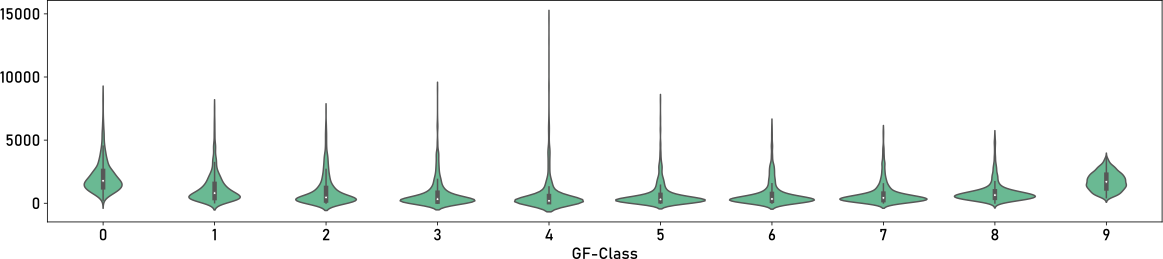
\includegraphics[width=\textwidth]{figures/gfs.pdf}
    \caption[Typical Gene Frequency Spectrum.]{Typical distribution of gene frequency classes. 10 Individuals simulated with $\theta = 1000$ and $\rho = 0.2$.}
    \label{fig:typical-gfs}
\end{figure}

The figure \ref{fig:typical-gfs} shows a typical distribution of gene frequency classes.
In this example, 10 individuals were simulated with a gene gain / gene loss rate of 1000 and 0.2 respectively.
The Kolmogorov-Smirnov test quantifies the difference between the simulated distribution and the observed value.
This is repeated for each gene frequency class.

Similar to the \ac{KS} approach, the \ac{KDE}-based direct approach fits a kernel density estimate with a Gaussian kernel to each distribution.
This results in a smooth approximation of the probability density function.
To evaluate how extreme the observed data point under the neutral evolution model is, we calculate a p-value by integrating the \ac{KDE} from the observed data point to either positive or negative infinity.
The integral represents the probability of observing a data point that is as extreme or more extreme than the observed value under neutrality.

In both the \ac{KS} test and the \ac{KDE} integration, the null hypothesis is that the two observed samples are drawn from the given distribution.
The two-tailed alternative hypothesis states that the distributions is different.

Importantly, the p-values derived from each gene frequency class are not independent.
This means that it is not possible to simply multiply them to determine the overall significance.
One solution is to use the smallest p-value, which is no longer a valid p-value in the traditional sense.
It is more likely to be smaller than the significance level, even if the null hypothesis is true for all tests.
This increased likelihood of Type I error is mitigated by directly implementing a Bonferroni correction:
\begin{equation}
    p_{\text{direct}} = \text{min}(p_{g^n_1}, ~ p_{g^n_2}, ~ ..., ~ p_{g^n_n}) \cdot n
\end{equation}

If this minimum p-value falls below our chosen significance threshold, we reject the null hypothesis of neutral evolution.
This rejection suggests that the observed \ac{GFS} could be influenced by factors other than neutral evolutionary processes, such as \ac{HGT}.

\subsection{Through a $\chi^2$-like Summary Statistic}\label{subsec:chi}
Through a $\chi^2$ -like summary statistics, we can directly measure the distance between the measured gene frequency spectrum $(g_1^n, ..., g_n^n)$, and its expected values under neutral evolution.
We define:

\begin{equation}
    \chi^2(g_1^n, ..., g_n^n) = \Sigma^n_{i=1} \frac{(g_i^n-\mathbb{E}[G_i^n])^2}{\mathbb{E}[G_i^n]}
\end{equation}
Following a similar approach, we generate many gene frequency spectra under a neutral evolutionary model.
We then compute a $\chi^2$-like statistics for each spectrum.
Unlike previous methods, this approach produces a single distribution allowing us to directly apply a \ac{KS}-test and fit a kernel density estimate.
As the $\chi^2$ value increases as the error from the expected values increases, only a one-tailed test is used.

The kernel density estimate shown in figure \ref{fig:pdf-cdf} characterises the \ac{PDF} of the $\chi^2$ values.
Together with the \ac{CDF}, a logarithmic transformation of it shows similarity to a normal distribution, although its shape is slightly skewed, indicating that the $\chi^2$ values follow a log-normal distribution.

\begin{figure}[]
    \centering
    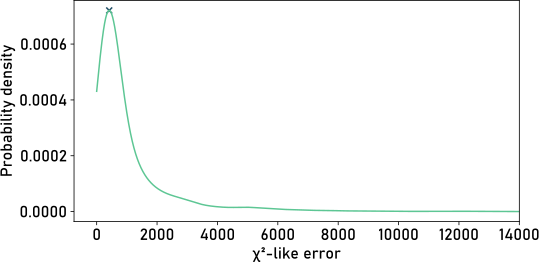
\includegraphics[height=3.5cm]{figures/pdf.pdf}
    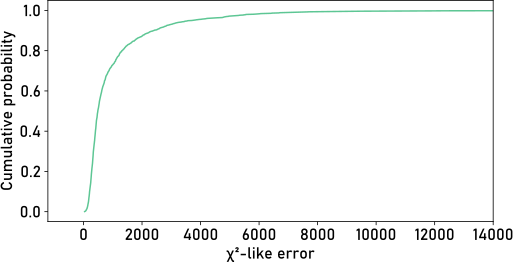
\includegraphics[height=3.5cm]{figures/cdf.pdf}
    \caption[Typical PDF and CDF.]{Typical Probability Density Function (left) and Cumulative Distribution Function (right) of $\chi^2$ values.}
    \label{fig:pdf-cdf}
\end{figure}
\newpage
To account for the variability observed between gene frequency classes, which is particularly pronounced at the boundaries ($g_1^n$ and $g_n^n$) compared to the centre, we introduce a weighting parameter to control the influence of each class.
This weight vector assigns relative importance to each gene frequency class.
By default, in the unweighted scenario, the weight vector is defined as $(w_0, w_1, \ldots, w_n)$, where each $w_i = 1$.
As these are relative weights, they must satisfy the condition $\sum_{i=0}^n w_i = n$.
The adapted $\chi^2$ -like summary statistic is now as follows:

\begin{equation}
    \chi^2(g_1^n, ..., g_n^n) = \Sigma^n_{i=1} \frac{(g_i^n-\mathbb{E}[G_i^n])^2}{\mathbb{E}[G_i^n]} w_i
\end{equation}

\section{Minimal Site Count}

While investigating the effect of the number of sites on the simulation runtime,
it became clear that a low number of sites is desirable in order to run multiple simulations efficiently and to obtain reliable neutrality test results.
However, in the infinite gene model, a high number of sites, ideally approaching infinity, is necessary as otherwise a gene gain event is likely to occur at a site where a gene already exists.
This includes gene gain events where the root ancestral state is `present'.
It is therefore desirable to find the minimum number of sites that will not significantly bias the resulting statistics.
An analytical and a computational approach have been used to do this.
For a single event the probability that a given event is a gene-gain is:
$$P_\theta = \frac{\theta}{\theta + \rho \cdot s}$$
with $s$ the total number of sites.
With that, the probability that at least one the $s$ sites is hit twice is:

\begin{equation}
    P_{\text{double}} = 1-(1-P_\theta^2)^s =  1-(1-(\frac{\theta}{\theta + \rho \cdot s})^2)^s
\end{equation}

\begin{figure}[h]
    \centering
    \includegraphics[width=0.6\textwidth]{figures/double_proba.pdf}
    \caption[Probability of double gene gain events.]{Probability that at least one double gene gain event is happening.}
    \label{fig:double-proba}
\end{figure}

The figure \ref{fig:double-proba} showed that double gene gain events remain likely, even for small gain/loss ratios, unless a very high number of sites ($>> 10^6$) is used.
The second approach looked at the effect on the $\chi^2$-like statistics.
Simulations were run with different number of sites ranging from $1000$ to $500000$.
Each simulation ($n = 10, \theta = 100, \rho = 0.1$) was repeated 1000 times.
For these simulations, the \ac{GFS} was recorded and the $\chi^2$-like statistic calculated and log-transformed.
The results were compared with a reference distribution assuming a site count of $10^6$, as the number of observed double mutations were low ($< 10$).
For a low number of sites ($s < 20000$), a t-test indicated significant deviations from the expected neutral model, as indicated by the very low p-values.
For higher $s$, the p-values increased and exceeded the $0.05$ threshold, indicating less deviation from the expected neutrality.
The table with all p-values can be found in appendix \ref{app:double-p-value}.
We therefore concluded that double gene gain can significantly bias the $\chi^2$-like statistical summary.


Despite these observations, a hard limit on the number of sites has not been implemented in order to maintain flexibility for the user.
Nevertheless, the number of double gain events is tracked to ensure the reliability of the results.
A warning is given if the frequency of these events exceeds 1\% of the total number of mutation events.

\subsection{Relocation of mutations}
Apart from as increasing the total number of sites, an alternative strategy is to relocate the double gene gain mutations.
In the case of recombination or gene conversion, different trees describe different segments of the genome.
Therefore, moving a mutation to an unused position could place it on a different tree and change its properties.
This is because mutations are more likely to occur twice in the same place on longer trees.
Consequently, the new position must be selected with the same bias, making random repositioning impractical.
Although this could be assessed by repositioning the mutation only within the bounds, this would drastically limit the number of mutations that could be repositioned.
Therefore, our implementation of random repositioning focuses only on scenarios without recombination or gene conversion.
This process involves extracting the tabular representation of the tree and creating a mask for double gene gain mutations based on the derived and parental states.
These identified mutations are then duplicated and mapped to a new, unused position and site.
To optimise computational efficiency, we access the data directly and create an array of all mutations / sites,
bypassing the resource-intensive creation of \mintinline{python}{MutationTableRow} and \mintinline{python}{SiteTableRow} objects.
While this is a fast and intuitive approach, it is limited by the number of possible new positions.
Thus, a \mintinline{python}{RuntimeError} is raised if the number of double mutations exceeds the number of free sites.

\newpage
\subsection{Genome Splitting}
An alternative approach to dealing with double gene gain events is to simulate with twice the number of sites.
This will double the number of mutations and approximately double the simulation time.
Following the simulation, we divide the mutations into a `left' and a `right' partition, ensuring an equal number of sites in each.
In the left partition, we eliminate all double gain mutations (i.e., gain mutations with gain mutations or `present' ancestral states as their parents).
On the right, we remove mutations that are not double gain mutations.
In addition, we reset the ancestral state drawn from the root distribution to `absent' to avoid sites marked as `present' without mutations.

Finally, we use the \mintinline{python}{tables.compute_mutation_parents()} function to correct any missing parental
relationships to ensure the integrity of the tree structure.
This allows us to reconstruct the tree without double mutations and similar features.

\begin{figure}[h]
    \centering
    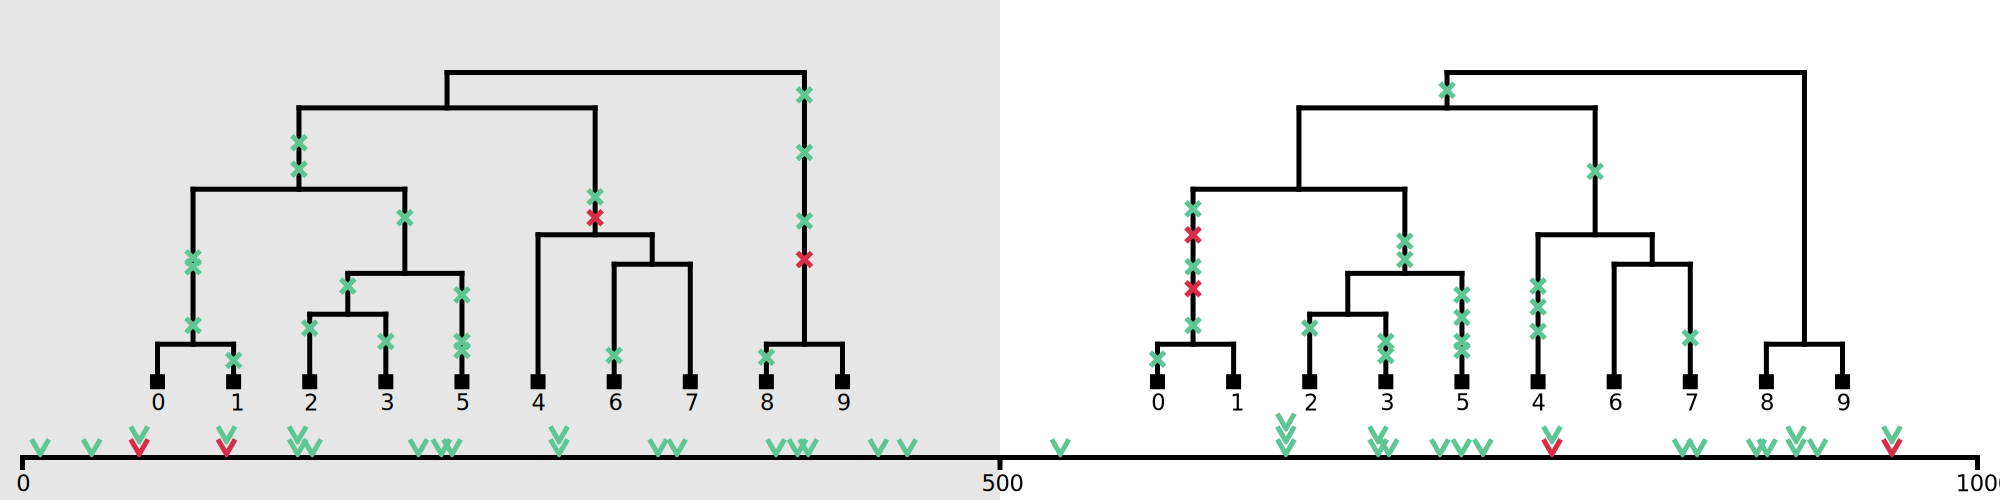
\includegraphics[width=\textwidth]{figures/tree_split_pre.pdf}\\
    \includegraphics[width=\textwidth]{figures/tree_split_post.pdf}
    \caption[Tree splitting for mutation relocation.]{Tree with mutations before (top) and after (bottom) splitting and removal of mutations.}
    \label{fig:tree-split}
\end{figure}

If, as in this example, a genome with 500 sites were desired, a simulation with 1000 sites would be used.
Here 42 mutations were simulated, 4 of which were double mutations.
On the left partition of the genome, all (2) double mutations were removed, while on the right partition only the double mutations (red) were kept.
While the genome has 1000 sites, it has the same number of present genes as a simulation with 500 under the \ac{IMG} model.

\section{Integration}
The gene gain and loss mutation model has been integrated with the customised \ac{HGT} ancestry and mutation simulation model to form a complete framework.
To provide a user-friendly interface, mutation relocation and tree fixation have also been added to this function.
Care had to be taken when relocating mutations as some sentinel mutations would be identified as double gene gain mutations.
An additional mask using the mutations' metadata has been introduced to account for this.
Due to its superior performance, the C implementation is used over the Python version whenever possible, especially when $\gamma = 0$ zero or when no \ac{HGT} events have been simulated.

\begin{table}[H]
    \label{tab:parameters}
    \begin{adjustbox}{width=\textwidth}
        \begin{tabular}{r|lll}
                     & Parameter                                      & Type                                     & Description                                                                                \\
            \hline
            $\theta$ & \mintinline{python}{theta}                     & \mintinline{python}{int}                 & Gene gain rate.                                                                            \\
            $\rho$   & \mintinline{python}{rho}                       & \mintinline{python}{float}               & Gene loss rate.                                                                            \\
                     & \mintinline{python}{ts}                        & \mintinline{python}{tskit.TreeSequence}  & \mintinline{python}{TreeSequence} to simulate gene gain and loss directly on this tree.    \\
                     & \mintinline{python}{hgt_edges}                 & \mintinline{python}{List[tskit.Edge]}    & List of HGT edges that can't be represented in the \mintinline{python}{TreeSequence}.      \\
            $n$      & \mintinline{python}{num_samples}               & \mintinline{python}{int}                 & Number of samples.                                                                         \\
            $s$      & \mintinline{python}{num_sites}                 & \mintinline{python}{int}                 & Number of sites in the genome.                                                             \\
            $\kappa$ & \mintinline{python}{gene_conversion_rate}      & \mintinline{python}{float}               & Gene conversion rate.                                                                      \\
                     & \mintinline{python}{recombination_rate}        & \mintinline{python}{int}                 & Recombination rate.                                                                        \\
            $\rho$   & \mintinline{python}{hgt_rate}                  & \mintinline{python}{float}               & Horizontal Gene Transfer rate.                                                             \\
                     & \mintinline{python}{ce_from_nwk}               & \mintinline{python}{str}                 & Tree structure in Newick format to follow during simulation.                               \\
                     & \mintinline{python}{ce_from_ts}                & \mintinline{python}{tskit.TreeSequence } & Tree structure in \mintinline{python}{TreeSequence} format to follow during simulation.    \\
                     & \mintinline{python}{check_double_gene_gain}    & \mintinline{python}{bool}                & Warning if more than 1\% of all events are double gene gain events.                        \\
                     & \mintinline{python}{double_site_relocation}    & \mintinline{python}{bool}                & Simulates with $2 \times $ \mintinline{python}{num_sites} and fixes double gain mutations. \\
                     & \mintinline{python}{relocate_double_gene_gain} & \mintinline{python}{bool}                & Repositions double gene gain mutations.                                                    \\
        \end{tabular}
    \end{adjustbox}
    \caption{Parameters of the \mintinline{python}{gene_model} function that combines the HGT ancestry simulation with the gene gain / loss model.}
\end{table}

\section{Estimating parameters for real world pangenomes}
To test the models' capabilities, we used real-world pangenomes, calculated the \ac{GFS} and optimised the simulation parameters using a \textit{Simplicial Homology Global Optimisation} and \textit{Differential Evolution} approach to match the simulated \ac{GFS} with the real ones.
Samples of multiple bacterial species we downloaded and processed by Hannah G\"otsch using \textit{PanX}.

\textit{PanX} is a software tool designed to streamline the construction and analysis of pan-genomes \cite{Ding_2017}.
It begins by using the \textit{DIAMOND} alignment algorithm to perform an all-against-all similarity search, identifying pairs of genes across the input genomes that have significant sequence similarity \cite{Buchfink_2014}.
These similarity results are then clustered using a Markov clustering algorithm, which groups genes that are likely to have a common evolutionary origin (orthologs).
As \textit{DIAMOND} focuses on proteins, \textit{PanX} has a separate process to identify and cluster non-coding genes such as ribosomal RNAs (rRNAs) using BLASTn.
To cope with the potential computational burden of analysing thousands of genomes, \textit{PanX} avoids direct all-against-all comparisons.
Instead, it clusters smaller subsets of genomes, then represents these clusters by `pseudo-genomes' and repeats this process hierarchically.
This strategy helps to maintain a near-linear growth in computational cost as the number of genomes increases.

\textit{PanX} constructs phylogenetic trees for each gene cluster using tools such as MAFFT (for alignment) and FastTree (for tree-building) \cite{Katoh_2002} \cite{Price_2010}.
These trees are carefully analysed to split gene clusters that may contain paralogs (genes related by duplication within a genome).
\textit{PanX} uses a combination of branch length thresholds and a `paralogy score' to finely separate orthologs into distinct groups.
It also has a process to address genes that may have been missed in the initial clustering, combining them based on sequence length and phylogenetic analysis.

Using alignments of core genes (present in all strains), \textit{PanX} builds a `core genome' phylogenetic tree using \textit{FastTree} and refines it using \textit{RaxML}.
This tree shows the overall evolutionary relationships between the strains.
Later, this tree is used to remove potential oversampling using \textit{PhyloThin}.

The thinned core genome trees and gene presence/absence matrices were exported and used for subsequent parameter estimation using the Simplicial Homology Global Optimisation algorithm.

The \ac{SHGO} algorithm is a method for efficiently identifying local minima in objective functions, especially when, as in our case, the function is costly to evaluate \cite{Endres_2018}.
For this we use the implementation of the \textit{SciPy} package \cite{scipy}.
As objective function we used the $\chi^2$ error of the mean \ac{GFS} of 24 simulations against the true \ac{GFS}.
This choice was a compromise between run time and variability of the error.
The algorithm uses concepts of simplicial integral homology and combinatorial topology to navigate complex problem landscapes,
which makes it useful for high-dimensional and complex applications such as exploring energy landscapes or, in our case, the $\chi^2$-like error for different parameters.
Of course this step assumes that the phylogenetic tree, computed by \textit{PanX} is correct.

\ac{SHGO} works by starting with the construction of a simplicial complex from the feasible search space.
This complex forms a topological abstraction where the vertices represent potential solutions and the simplicial links illustrate possible optimisation paths.
By approximating the homology groups of this complex, \ac{SHGO} is able to map the structure of the search space and pinpoint areas likely to contain local minima.
The search space is defined by bounds that we set to:

\begin{table}[h]
    \begin{adjustbox}{width=\textwidth}
        \begin{tabular}{llll}
            Parameter & start  & stop                               & Description                    \\
            \hline
            $\theta$  & 0.1    & average number of genes $\times 3$ & Gene gain rate.                \\
            $\rho$    & 0.0001 & number of samples                  & Gene loss rate.                \\
            $\kappa$  & 0      & 0.01                               & Gene conversion rate.          \\
            $\gamma$  & 0      & 0.01                               & Horizontal Gene Transfer rate. \\
            recomb    & 0      & 0.01                               & Recombination rate.
        \end{tabular}
    \end{adjustbox}
    \caption{Parameter search-space.}
\end{table}

based on our previous experience and runtime feasibility.

The algorithm uses intelligent sampling methods based on the vertices of the simplicial complex, guided by Sperner's lemma.
This lemma helps to approximate locally convex subdomains that are likely locations of local minima, significantly reducing the number of function evaluations required.

The other optimisation technique we used is the \ac{DE} approach by Storn and Price \cite{Diff_Evo_Storn_1997} which finds an optimal solution by evolving a population of candidate solutions over time.
Differential Evolution involves four main steps: initialization, mutation, crossover, and selection.
Initially, a population of $15$ candidate solutions is randomly generated, within our search space. We use the same bounds as in the \ac{SHGO} approach.
Each candidate solution, also called an individual, is represented as a vector.
Once the initial population is established, the algorithm proceeds to the mutation step.
In this phase, for each candidate solution in the current population, a mutant vector is generated.
This is done by selecting three distinct individuals from the population and combining them by adding the weighted difference between two of these individuals to the third one.
The mutation is followed by the crossover step which aims to increase the diversity of the population by randomly combining components of the mutant vector with the candidate vector to create a trial vector.

Finally, in the selection step, the trial vector is compared to the target vector based on their fitness values, which are determined by the objective function being minimised.
If the trial vector has a better fitness value than the candidate vector, it replaces it in the population.
This ensures that the population evolves towards better solutions over successive generations.

Once the minimisation process had converged, the parameters were recorded and further refined using a \ac{DS} approach.
This additional step is necessary as both \ac{SHGO} and \ac{DE} algorithms excel at exploring the wider $\chi^2$ value landscape,
but struggle in the final, local optimisation.

For this step, the number of simulations per evaluation of the objective function was increased
from 24 to 48 in order to reduce the variability of the $\chi^2$ like value.
The result of this process is a list representing several gene frequency spectra,
providing a distribution and $\chi^2$ like measurement indicating the fit of the simulated parameters to the true parameters.

\cleardoublepage

% !TeX spellcheck = en_GB
\chapter{Results and Discussion}\label{kap:results}
\section{Effect of Gene Conversion on the GFS}
The effect of gene conversion on the gene frequency spectrum becomes most apparent when simulations are performed on a fixed tree with a recognisable \ac{GFS} pattern.
In our constructed tree (figure \ref{fig:tree-gc-loss}) with three distinct clades (C1: individuals 0-3, C2: individuals 4-7, C3: individuals 8-9),
the two leftmost clades consist of four individuals each, while the right clade consists of only two.
Due to numerous gene gain events along the long branch from node 18 to 17, we expect these genes to spread across the entire left side, resulting in a \ac{GFS} peak at class 8.
Similarly, along the branches 17 to 15 and 17 to 16, the gene gain affects the entire clade, resulting in a \ac{GFS} peak at class 4.
The same principle applies to the 18 to 14 branch, but for the smaller clade, resulting in a peak at class 2.
Genes present in all 10 individuals are less likely to stem from regular event as this would require at least two gene gain events at the same site on different branches, but rather stem from the ancestral state.
As the \ac{GFS} includes those and does not distinguish between those genes we expect another peak at class 10.
While it is easy to infer the GFS from a tree structure, it is not possible to do the inverse.


The introduction of a single gene conversion event causes a gene in a few individuals to follow an alternative phylogenetic tree.
This is illustrated by the light green segment / branches in the figure that oppose to the dominant tree in dark blue.
Due to the long edge from 18 top GC1 an increase of the peak Gene Frequency Class 6 would be expected.


As gene conversion increases, more genome segments are determined by different trees, disrupting the effect of the initial structure.
Consequently, the expected \ac{GFS} across different fixed trees with gene conversion converges towards the expected \ac{GFS} of random trees under neutral evolution.
Nevertheless, certain features persist even with increased gene conversion rates, such as the peak at class 4 and class 10.
These would require numerous gene conversion events to counteract the strong influence of long edges and the root probability of the ancestral state.
This is visible in figure \ref{fig:tree-gc-loss} (right) which depict the \ac{GFS} for different gene conversion rates and the mean $\chi^2$-like error.

\begin{figure}[h]
    \centering
    \begin{minipage}{0.49\textwidth}
        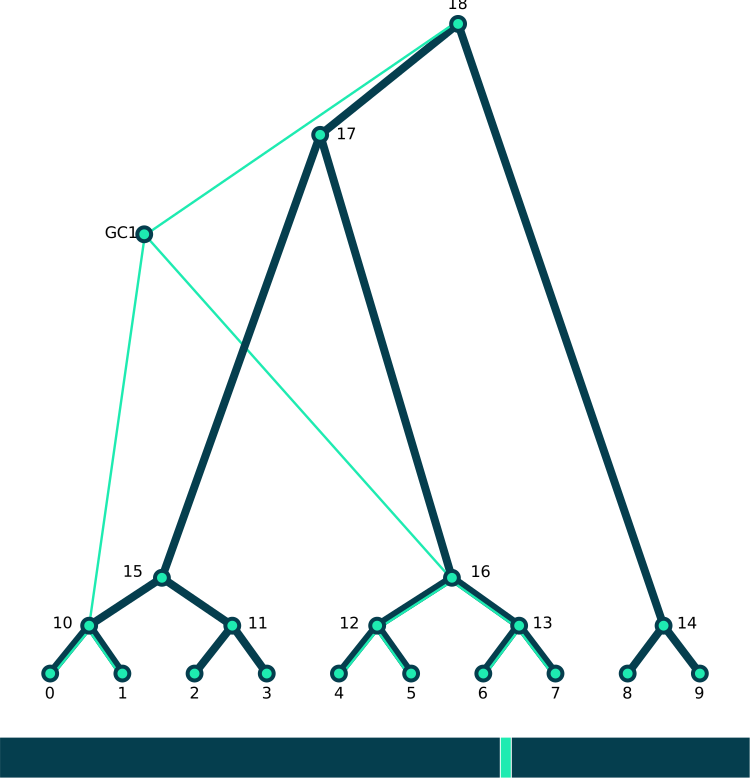
\includegraphics[width=\textwidth]{figures/effect_on_gfs/tree_with_gc.pdf}
    \end{minipage}
    \begin{minipage}{0.49\textwidth}
        \hfill\includegraphics[width=0.99\textwidth]{figures/effect_on_gfs/gfs_gc.pdf}\\
        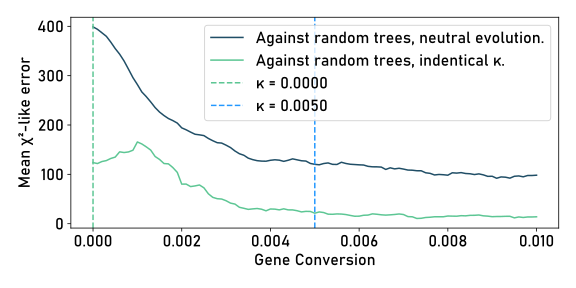
\includegraphics[width=\textwidth]{figures/effect_on_gfs/gfs_gc_factor.pdf}
    \end{minipage}
    \caption[Effect of gene conversion on the GFS.]{Tree with one gene conversion event (left), its GFS for different gene conversion rates (top right) and
        its respective $\chi^2$-like error (bottom right).}
    \label{fig:tree-gc-loss}
\end{figure}

When inspecting the non-normalized \ac{GFS} of simulations with a fixed tree, it apparently it does not exactly match the expected \ac{GFS} of neutral random trees.
Instead, it reflects its shape but is slightly shifted based on the gene gain/loss parameters.
This shift is caused by the emergence of new lineages due to gene conversion, which increases the time to coalescence for all lineages.
As a result, the total potential for gene gain / loss events is increased.
The $\chi^2$-like error between the mean \ac{GFS} and the expected \ac{GFS} highlights this discrepancy.
Initially, the error drops to a low level but never reaches zero.

\section{Effect of HGT on the GFS}
\begin{figure}[h]
    \centering
    \includegraphics[width=0.49\textwidth]{figures/effect_on_gfs/gfs_hgt.pdf}
    \includegraphics[width=0.49\textwidth]{figures/effect_on_gfs/gfs_hgt_levels_2.pdf}
    \caption[Effect of HGT on the GFS.]{GFS for different HGT rates (left) on a fixed tree and on random trees (right).}
    \label{fig:hgt-loss}
\end{figure}

A high value of $\gamma$ shifts the gene frequency spectrum to the right, indicating that most genes are present at high frequency resulting in a characteristic \reflectbox{L} shape.
This means that when new individuals are sequenced, it is unlikely that new genes will be discovered that were not previously observed.
When a fixed tree is used, a similar effect to gene conversion is expected.
Along with the loss of characteristic features of the simulated tree, a shift to the right is expected, resulting in a smaller peak at lower gene frequency classes.
This is due to new edges introduced by horizontal gene transfer events changing the original tree structure.
This effect is visible in figure \ref{fig:hgt-loss}.

The increase in gene frequency is due to the nature of \ac{HGT}, where any gene acquisition in a lineage, whether by vertical inheritance or \ac{HGT}, is counted as a gain.
This effect is clearly visible in figure \ref{fig:hgt-loss} for simulations without tree fixation.

\section{Neutrality test robustness}
The properties of the neutrality test differ between the $\chi^2$ approach and the direct approach.
Understanding these differences helps to interpret test results and to determine the situations in which each approach may be most informative.

By relying on the minimum p-value across all \ac{GFS} classes, the direct approach is sensitive to small changes within individual classes.
Small variations in the underlying parameters ($\theta, \rho, \gamma$ and $\kappa$) can lead to pronounced changes, especially at the edges of the \ac{GFS} in classes $1$ and $n$.
The direct approach also shows reduced sensitivity to overall upward or downward shifts in the GFS, as these large changes may not significantly alter individual class probabilities.
These changes are captured by the $\chi^2$ approach by summing the respective errors.

\subsection{With neutral evolution as reference}
We assessed the robustness of our model by calculating the mean likelihood values and 90\% percentiles obtained from multiple neutrality tests.
This provides a measure of the stability of the test under different assumptions about evolution.
A reference distribution was generated by sampling the \ac{GFS} of 5000 simulations under neutral parameters.
Then 25 simulations were run for each step in our list of desired parameters (table \ref{app:robust-param}, figure \ref{fig:robust_gc0}).

The plots of these results include a vertical blue line indicating the true parameters used in the neutral reference simulation:

\begin{itemize}
    \item \textbf{Gene Gain} ($\theta$): Tests around theta perform consistently well, forming the expected bell curve around the true parameter values.
          Deviations as large as 1000 lead to significant drops in p-values (below 0.1).
    \item \textbf{Gene Loss} ($\rho$): A similar pattern can be observed for Rho. Here we see a saturation effect, as at high gene loss values the effect is less pronounced,
          as most events occur at sites where no gene is already present.
    \item \textbf{Gene Conversion} ($\kappa$): As higher gene conversion rates shift the gene frequency spectrum towards that expected from random tree models, the variance of the \ac{GFS} decreases.
          As a result, the tests do not detect deviations due to increased gene conversion rates.
          However, if a simulation with gene conversion ($\kappa$ = 2) is used as a reference, it is possible to detect values originating from a simulation with low gene conversion.
    \item \textbf{HGT} ($\gamma$): The effect of \ac{HGT} is clearly visible, with a half bell curve around the true value.
          As the effect of \ac{HGT} is strong on individual GF classes as well as all classes together, it is well picked up by the $\chi^2$ based and direct test
\end{itemize}
\begin{figure}[]
    \centering
    \begin{minipage}{0.49\textwidth}
        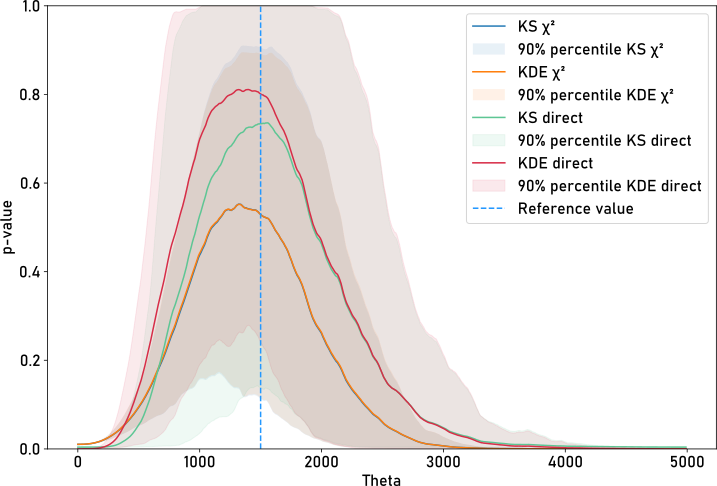
\includegraphics[width=\textwidth]{figures/neutrality_test/gc_0_theta.pdf}\\
        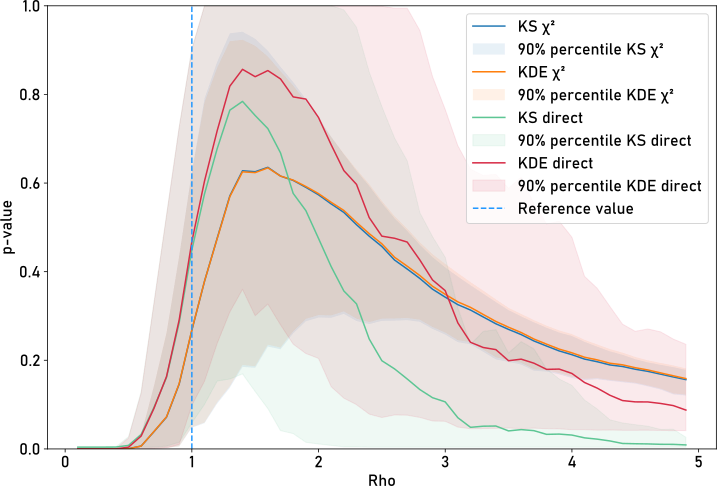
\includegraphics[width=\textwidth]{figures/neutrality_test/gc_0_rho.pdf}
    \end{minipage}
    \begin{minipage}{0.49\textwidth}
        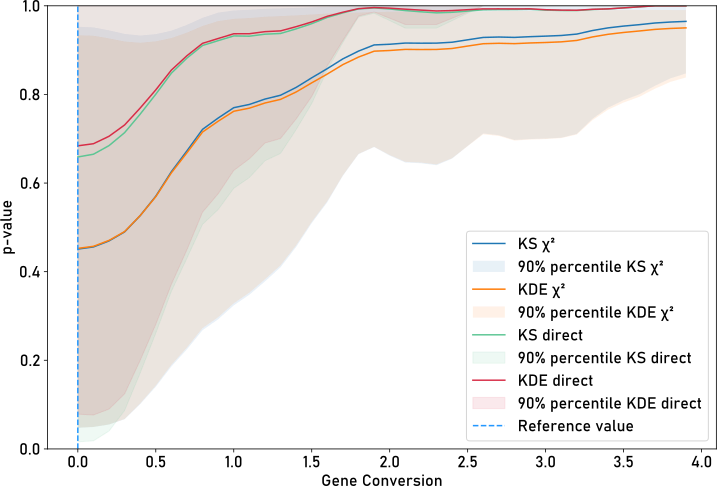
\includegraphics[width=\textwidth]{figures/neutrality_test/gc_0_gc.pdf}\\
        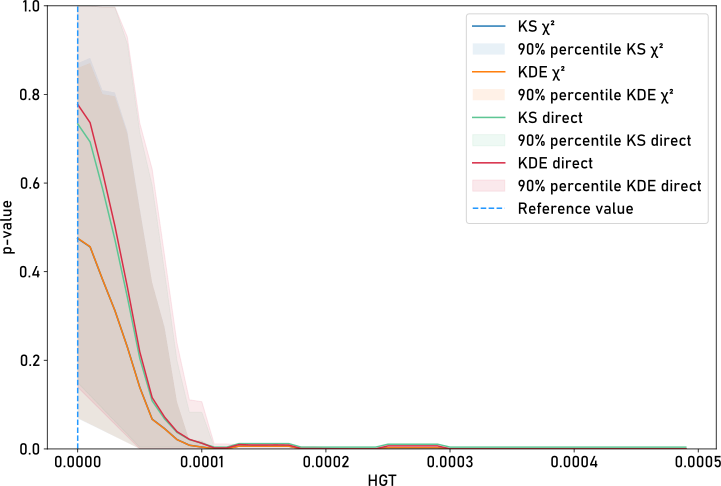
\includegraphics[width=\textwidth]{figures/neutrality_test/gc_0_hgt.pdf}
    \end{minipage}
    \caption[Robustness of the neutrality test for $\kappa = 0$.]{Robustness of the neutrality test for different $\theta$ (top left), $\rho$ (bottom left), $\kappa$ (top right), $\gamma$ (bottom right) values
        with a neutral evolution as reference.}
    \label{fig:robust_gc0}
\end{figure}

\subsection{Non-neutral evolution as reference}

As the neutrality test is based on a simulated reference distribution it is also possible to test against an evolution with gene conversion or \ac{HGT}.
When considering non-neutral evolutionary processes, the expected gene frequency spectrum distribution must be adjusted accordingly.
In the following test, the reference distribution was obtained by simulating with $\gamma = 0.0001$.
A total of 5000 samples were recorded.
Similar characteristics are observed for changes in $\theta$ and $\rho$: a bell curve around the true $\theta$ value and a tail for $\rho$ due to the saturation effect.
See figure \ref{fig:robust_hgt}.
The difference between the \ac{KDE}-smoothed and \ac{KS}-based $\chi^2$ test appears to be due to rare outliers.
These outliers affect the smoothing process, resulting in a wider distribution and therefore a less effective test.
For \ac{HGT}, the test is able to distinguish whether the new data stems from a simulation with less or no \ac{HGT}, and shows a right tailed bell curve.
This left part of the curve reflects the test results from the neutral evolution, as it is the inverted version if it.
For higher \ac{HGT} values, the sensitivity decreases and significantly higher \ac{HGT} values are required.
The reason for this is that the reference \ac{HGT} value of 0.0001 already has a strong effect on the gene frequency spectrum,
and the relative change for higher values is small as the effect saturates.
A similar pattern was observed for simulations with gene conversion ($\kappa = 2$, figure \ref{fig:robust_hgt} bottom right) as a reference.
Here the test is able to detect \ac{GFS} from the simulation with less gene conversion.
Detection of higher values of $\kappa$ is not possible, as the effect of gene conversion saturates after pushing the \ac{GFS} to the expected \ac{GFS} for random trees.

The complete list of measurement can be found in appendix \ref{app:robust_gc}.

\begin{figure}[h]
    \centering
    \begin{minipage}{0.49\textwidth}
        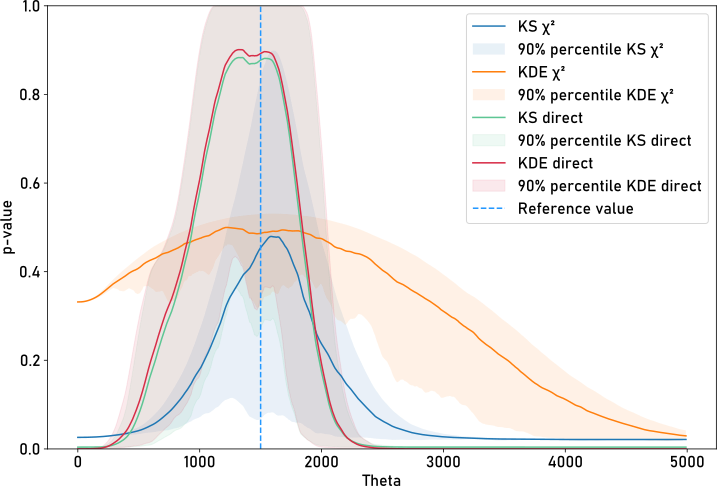
\includegraphics[width=\textwidth]{figures/neutrality_test/hgt_0.0001_theta.pdf}\\
        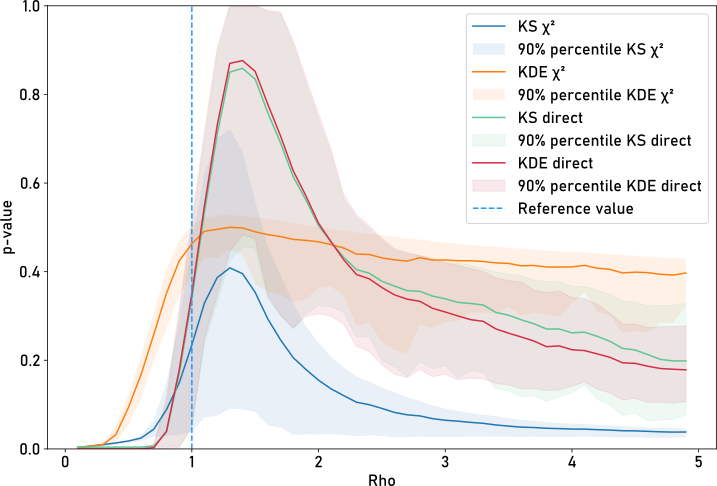
\includegraphics[width=\textwidth]{figures/neutrality_test/hgt_0.0001_rho.pdf}
    \end{minipage}
    \begin{minipage}{0.49\textwidth}
        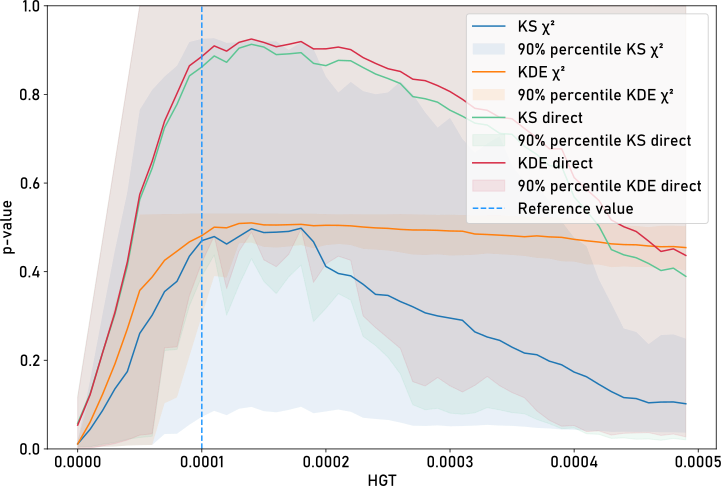
\includegraphics[width=\textwidth]{figures/neutrality_test/hgt_0.0001_hgt.pdf}\\ %hgt
        \includegraphics[width=\textwidth]{figures/neutrality_test/gc_2_gc.pdf} %gc2
    \end{minipage}
    \caption[Robustness of the neutrality test for $\gamma = 0.001$ and $\kappa = 2$ as reference.]{Robustness of the neutrality test for different $\theta$ (top left), $\rho$ (bottom left), $\kappa$ (top right), $\gamma$ (bottom right) values
        with $\gamma = 0.001$ (top / bottom left, top right) and $\kappa = 2$ (bottom right) as reference.}
    \label{fig:robust_hgt}
\end{figure}


\section{Runtime}
To ensure that the new gene model has a feasible runtime - necessary due to the multiple runs required for neutrality estimation - we investigated the effect of different parameters.

Simulations without \ac{HGT} are using the underlying C implementation, while those with \ac{HGT} are using a pure Python implementation.
This difference is expected to lead to significant differences in runtime.
To capture this effect, we timed a wide range of values for the parameters $n$, $s$, $\theta$, $\rho$ and $\kappa$ with a \ac{HGT} rate $\gamma$ set to 0 and 0.001.
Each parameter was tested in isolation, i.e. only one parameter was varied while the others were held constant at their default settings.

The parameters, their default values and their ranges tested were as follows:
\begin{table}[h]
    \begin{adjustbox}{width=\textwidth}
        \begin{tabular}{r|lllll}
            Parameter & Min  & Max    & Step   & Default    & Description                    \\
            \hline
            $n$       & 0    & 10000  & 10     & 10         & Number of samples.             \\
            $s$       & 1000 & 100000 & 100    & 10000      & Number of sites.               \\
            $\theta$  & 0    & 1000   & 1      & 100        & Gene gain rate.                \\
            $\rho$    & 0.01 & 0.5    & 0.001  & 0.1        & Gene loss rate.                \\
            $\kappa$  & 0    & 2      & 0.01   & 0          & Gene conversion rate.          \\
            \hline
            $\gamma$  & 0    & 0.005  & 0.0005 & 0 / 0.0001 & Horizontal Gene Transfer rate.
        \end{tabular}
    \end{adjustbox}
    \caption{Runtime analysis parameters.}
\end{table}

A total of 100 simulations were run for each step within a parameter's range, and run times were recorded.
Some parameter combinations were also tested to identify potential pairwise dependencies.
The individual plots (figure \ref{fig:runtime}) show the mean runtimes and the 90th percentiles.
Figures presenting the remaining parameters, simulation with HGT and the first difference of the runtimes are shown in the appendix \ref{app:runtime}.
As inferred from the implementation, the runtime follows a mostly linear dependence on problem and parameter size.

\begin{itemize}
    \item \textbf{Number of samples}: Runtime anomalies were observed for certain sample sizes, particularly around 500 for the C implementation.
          Initial hypotheses suggested that these anomalies might be due to default memory allocations or processor cache limitations.
          However, tests on different processors, regardless of L2/L3 cache size, showed similar increases at these sample sizes.
          Thermal throttling or switching from performance to efficiency cores was considered but ruled out due to the consistent runtime jumps at these specific points.
          Given the small impact of these anomalies and their absence in the Python version, they were ignored for the remainder of the study.

    \item \textbf{Number of genes}: The graphs show an almost linear increase in runtime as the number of genes increases, with the difference showing a slightly super-linear trend.
          With more genes, more positions have to be tracked, causing the increase.

    \item \textbf{Gene Gain} ($\theta$): Both graphs and their derivatives show a stable linear growth in runtime with increasing theta, reflecting the additional computational load of more gene gain events and the resulting increase in the number of lines to track.

    \item \textbf{Gene Loss} ($\rho$): A lower rho value means fewer gene loss events, resulting in more lines to simulate. As rho increases, fewer lines need to be simulated due to more frequent gene losses.
          However, at a certain point, simulating gene loss events takes longer than the time saved by eliminating lines, leading to a linear increase in run time.
          To fully understand the interaction between rho and theta, we plotted the execution time over a range of their combinations and ratios.

    \item \textbf{Ratio of $\rho$ to $\theta$}: The runtime for different ratios of $\theta$ and $\rho$ is presented in figure \ref{app:theta-rho-heatmap}.
          The effect of $\rho$ on runtime initially decreases execution time, followed by a linear increase as $\rho$ increases.
          In this analysis, the parameter range was set from 0 to 10,000 in steps of 100 for $\theta$ and 0 to 1 in steps of 0.01 for $\rho$.
          All possible combinations were measured, and the parameter grid was shuffled to reduce the impact of sorting bias.
          Outliers in the heatmap are likely due to measurement methods, as there is no clear pattern.\\
          \newpage
    \item \textbf{Gene Conversion} ($\kappa$): This parameter has a significant effect on running time, with a more than linear increase observed.
          Each gene conversion event introduces a new lineage into the population, increasing the number of generations required to reach the most recent common ancestor.

    \item \textbf{HGT} ($\gamma$): Similarly to gene conversion, this parameter has a strong effect on run time. Each \ac{HGT} event creates a new lineage that must be tracked and post-processed, leading to a superlinear increase in runtime.
\end{itemize}

Overall, these results highlight the impact of the number of lineages on the runtime and the need for a C implementation.
\begin{figure}[H]
    \begin{flushright}
        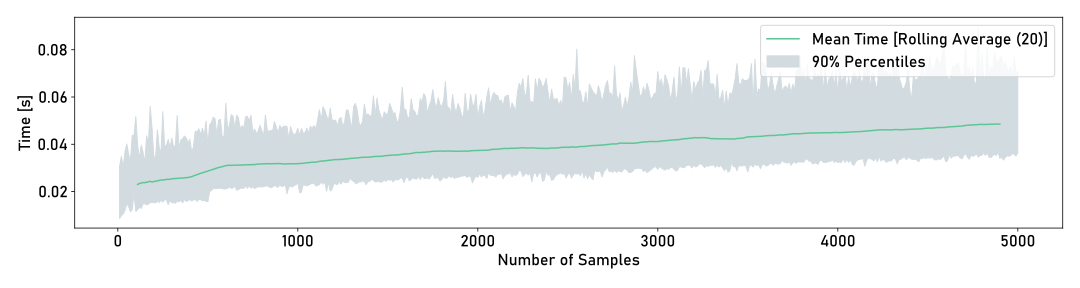
\includegraphics[width=\textwidth]{figures/runtime/num_samples.pdf}\\
        \includegraphics[width=\textwidth]{figures/runtime/num_sites.pdf}\\
        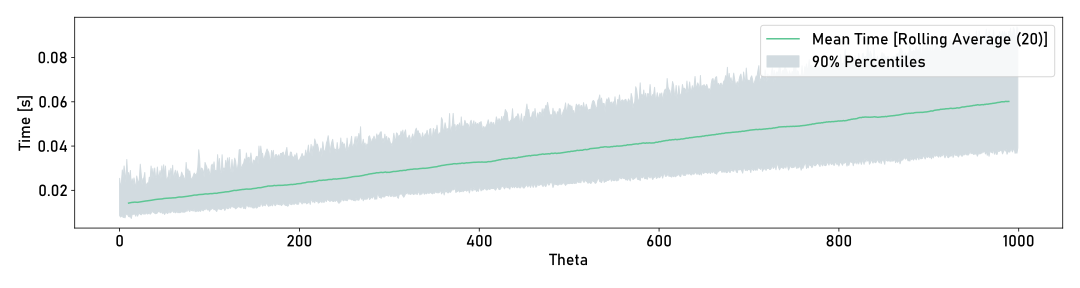
\includegraphics[width=\textwidth]{figures/runtime/theta.pdf}\\
        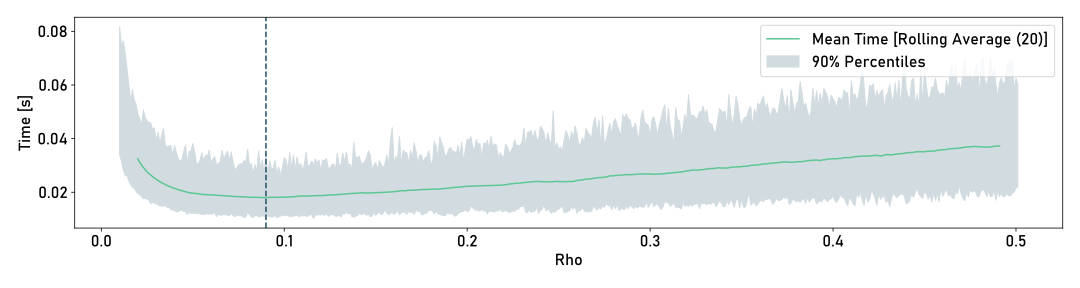
\includegraphics[width=\textwidth]{figures/runtime/rho.pdf}\\
    \end{flushright}
    \centering
    \caption[Runtime without HGT.]{Runtime of \mintinline{python}{gene_model} for different number of samples, number of sites, $\theta$ and $\rho$ rates
        for simulations without HGT.}
    \label{fig:runtime}
\end{figure}

\section{Estimating parameters for real world pangenomes}
\begin{figure}[H]
    \centering
    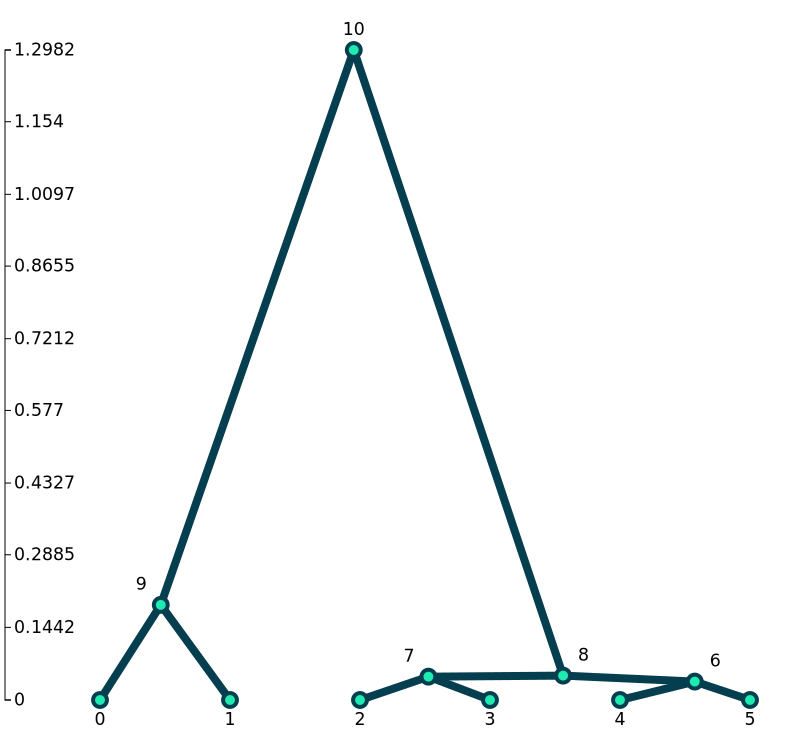
\includegraphics[width=0.49\textwidth]{figures/fitted_gfs/803.pdf}
    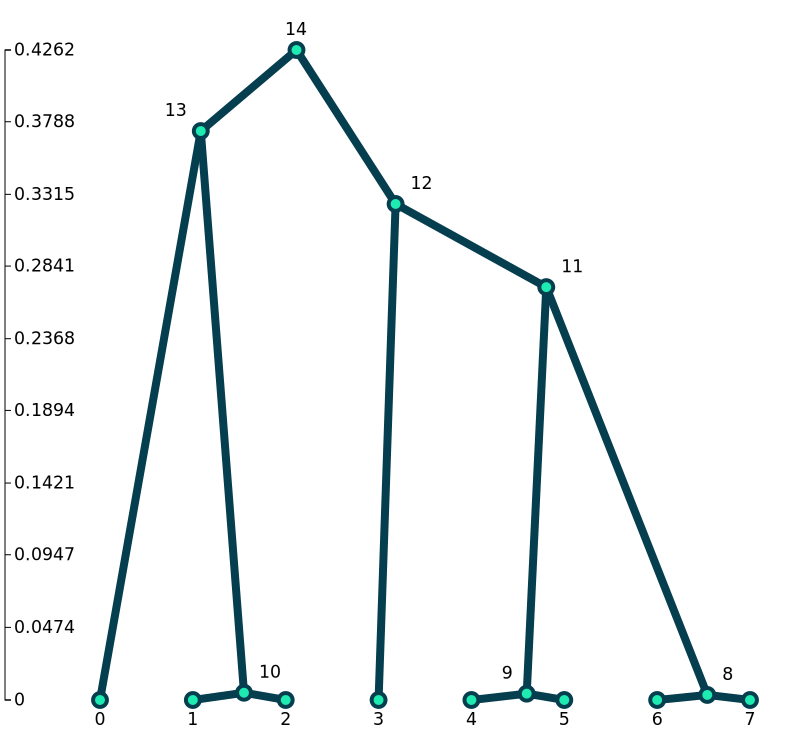
\includegraphics[width=0.49\textwidth]{figures/fitted_gfs/985002.pdf}\\
    \includegraphics[width=0.49\textwidth]{figures/fitted_gfs/1492.pdf}
    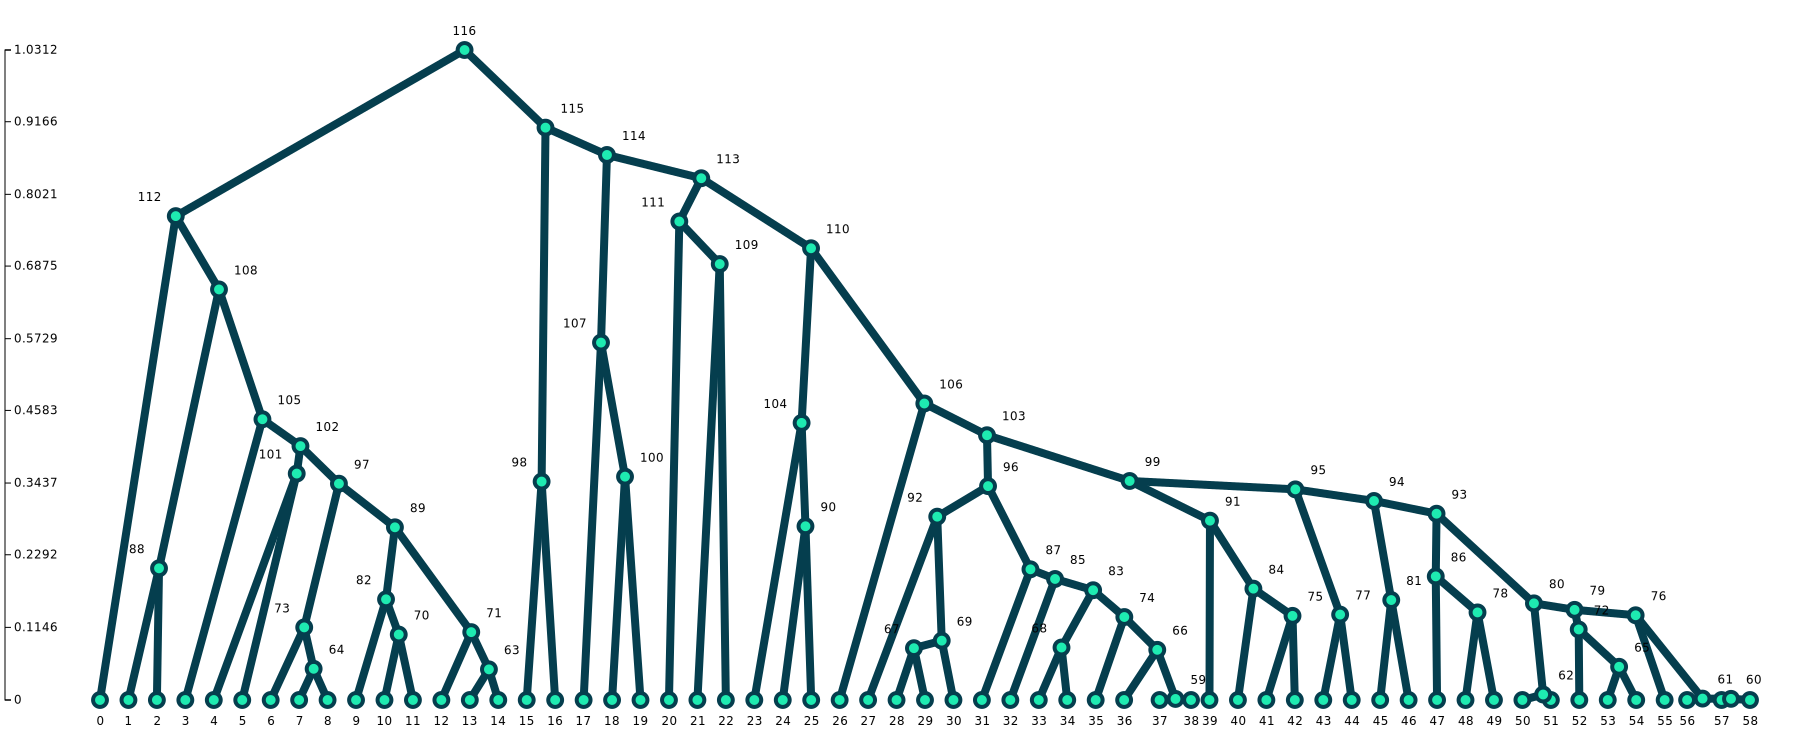
\includegraphics[width=0.49\textwidth]{figures/fitted_gfs/9.pdf}\\
    \caption[Fitted GFS for real-world pangenomes.]{True and simulated GFS for Bartonella quintana (top left), Staphylococcus argenteus (top right), Clostridium butyricum (bottom left), Buchnera aphidicola (bottom right).}
    \label{fig:fitted-gfs}
\end{figure}
With optimised parameters, our model successfully simulated matching GFS for most pangenomes but failed for some.
Although fitting is possible, as discussed in the previous section, it is slow due to the current Python-only implementation.
Therefore, we only used low sample count datasets.

Bartonella quintana, chosen due to its known high horizontal gene transfer rate \cite{Bartonella}.
Only 6 samples were present.
The fit is excellent, with a $\chi^2$ like error of 51 and an expected high resulting \ac{HGT} parameter of 0.003.
This would correspond to a rate of 30 if we rescale it by the number of sites.
As the used phylogenetic tree is balanced and the \ac{HGT} effect is strong, a characteristic \reflectbox{L} shape is visible.
An overview with all phylogenetic trees can be found in appendix \ref{app:panX-trees}.
\\
In addition, we selected another strain with slightly more samples where a high \ac{HGT} rate was expected.
We chose Staphylococcus argenteus as its part of the S. aureus related complex.
This strain had a similar \ac{HGT} value of 0.004
The fit is acceptable with a $\chi^2$ like error of 1170 and the significant right-shift of the \ac{GFS}
towards many high-frequency genes can be seen in the figure \ref{fig:fitted-gfs}.
It is important to note that the $\chi^2$ like error is not normalised and thus can't be compared directly between samples \ref{subsec:chi}.

In order to assess the model's capacity to handle the significant influence of the underlying phylogenetic tree,
we selected Clostridium butyricum, which exhibits a peak in the gene frequency class 9.
Despite the successful identification of parameters that resulted in matching \ac{GFS} for all other classes,
the optimisation algorithm was unable to identify parameters that replicated the peak in class 9.
This resulted in a $\chi^2$ line error of 749.
It is our hypothesis that the optimisation algorithm became trapped in local minima.
Local minima are particularly likely to occur when testing high gene conversion or \ac{HGT} rates.
The strong influence of these factors on the \ac{GFS}'s shape can significantly improve the $\chi^2$ like error in the first step,
but then also prevents the algorithm from identifying better parameters, as further changes to other parameters will have minimal impact.

As a representative example with a low rate of \ac{HGT} and a limited number of genes Buchnera aphidicola was chosen \cite{Buchnera}.
Unfortunately, due to its 59 samples, it resulted in a longer optimisation time, leading to unpolished parameters with a poor score. Here the fit resulted in a $\chi^2$ error of 701.
As the optimisation process had to be aborted due to the long run time and lack of computational resources, and as the results improved over time, we are optimistic that the fit could have been significantly better.

Differential Evolution proved to be significantly better than either \ac{SHGO} or
simple \ac{DS} for global optimisation. While \ac{DE} efficiently found reasonably good parameters for the first two samples in less than 1000 steps, \ac{SHGO} required over 2000 steps, leading to an impractically long runtime.

Therefore, after testing Bartonella quintana and Staphylococcus argenteus, we used \ac{DE} exclusively.
Locally, Downhill Simplex performs better than \ac{DE} and converges to a minimum faster.
Although \ac{DS} does not guarantee a global minimum, the variance of the local error is larger than the error itself, blocking any further minimisation.
This would be solved by using more simulations for each optimisation step to achieve a more stable $\chi^2$ like error, which would ultimately result in an impractical runtime.

\cleardoublepage

% !TeX spellcheck = en_GB
\chapter{Summary}
This thesis investigates the dynamics of Horizontal Gene Transfer (HGT) in bacterial populations, with a particular focus on the effects on the Gene Grequency Spectrum (GFS).
Traditional simulation models of genetic evolution based on clonal inheritance often overlook the effects of lateral gene flow introduced by HGT.
This research aims to integrate HGT into existing models to improve their accuracy and predictive power.

The mutation model of \textit{msprime} was extended by incorporating the concept of gene gain and loss based on the Infinitely Many Genes (IMG) model.
By moving the double gene gain mutation to unused sites, the problem of having a finite number of sites that would conflict with the IMG was mitigated.
This extension of \textit{msprime} allowed the simulation of gene frequency spectra and the development of a neutrality test to assess whether a GFS results from a neutral evolutionary process.

Ancestry and mutation simulation was further improved by introducing mechanisms for tree fixation and HGT.
This adaptation involved modifying the built-in ancestry simulation to create a new single-gene lineage for each HGT event, and adjusting the mutation algorithm to correctly place mutations while accounting for the potential influence of HGT.
This allowed the effects of HGT on the GFS to be studied.

The model was applied to real-world pangenome data from NCBI. Parameters were optimised using Simplicial Homology Global Optimisation (SHGO) and Differential Evolution (DE) to achieve a good fit between simulated and observed genetic patterns.
This was mostly achieved.

The extended \textit{msprime} and \textit{tskit} tools provide a robust framework for simulating and analysing genetic evolution, leading to more accurate predictions of evolutionary outcomes.
The results highlight the important role of HGT in microbial evolution and show that genetic uniformity can be rapidly introduced by lateral gene flow.

However, the model has two important limitations: it assumes constant rates of gene gain and loss, which may not reflect temporal variation, and the interaction between gene conversion and HGT increases the number of lineages, resulting in an infeasible runtime for large-scale simulations.
In addition, the pure Python implementation is not suitable for large-scale parameter estimation and simulation.

Future research should explore more dynamic models that account for varying rates of gene gain and loss over time, and provide a C implementation with an improved method for simulating gene conversion and HGT simultaneously.
This would allow the model to be fully integrated into \textit{msprime}.

This work has provided a framework for simulating the impact of HGT on genetic diversity in bacterial populations.

\cleardoublepage
% Anhaenge wieder mit roemischer Nummerierung
\pagenumbering{roman}
\setcounter{page}{1}
\addcontentsline{toc}{chapter}{Appendix}
\chapter*{Appendix\markboth{APPENDIX}{APPENDIX}}
\section{Influence of Double Gene Gain Events}\label{app:double-p-value}
The influence of double gene gain events on low gene-count simulations with 10 samples and$\theta = 100, \rho = 0.1$.
The $\chi^2$-like values for simulations with less than 20000 genes show a significant deviation from the reference.

\begin{table}[H]
    \begin{tabular}{l|l|c}
        Number of sites & P Value  & Significant \\
        \hline
        1000            & 2.21e-05 & x           \\
        2000            & 8.16e-21 & x           \\
        5000            & 3.40e-09 & x           \\
        10000           & 8.59e-05 & x           \\
        20000           & 0.13     &             \\
        50000           & 0.31     &             \\
        100000          & 0.78     &             \\
        200000          & 0.80     &             \\
        500000          & 0.12     &
    \end{tabular}
    \caption{Effect of double gene-gains on the log-transformed $\chi^2$-like values for low number of sites simulations.}
\end{table}
\newpage
\section{Neutrality Test Robustness}
\begin{table}[h]
    \centering
    \begin{tabular}{r|llll}
        Parameter & start & stop   & step    & default \\
        \hline
        $\theta$  & 0     & 5000   & 10      & 1500    \\
        $\rho$    & 0.1   & 5      & 0.1     & 1       \\
        $\kappa$  & 0     & 4      & 0.1     & 0       \\
        $\gamma$  & 0     & 0.0005 & 0.00001 & 0
    \end{tabular}
    \caption{Neutrality test robustness parameters.}
    \label{app:robust-param}
\end{table}

\begin{figure}[H]
    \centering
    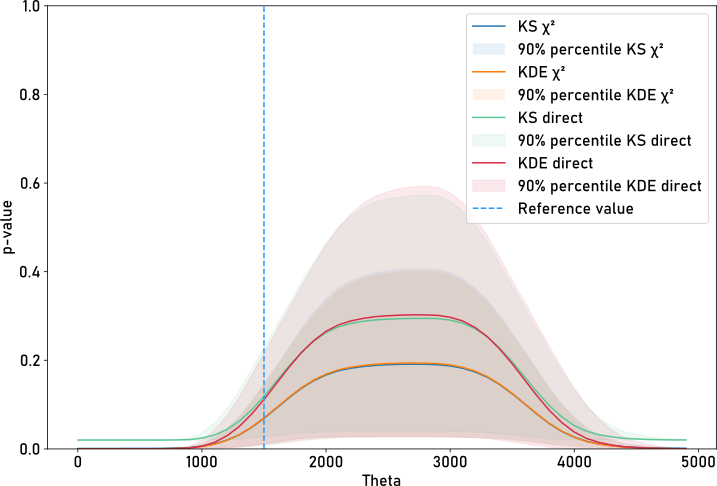
\includegraphics[width=0.49\textwidth]{figures/neutrality_test/gc_2_theta.pdf}
    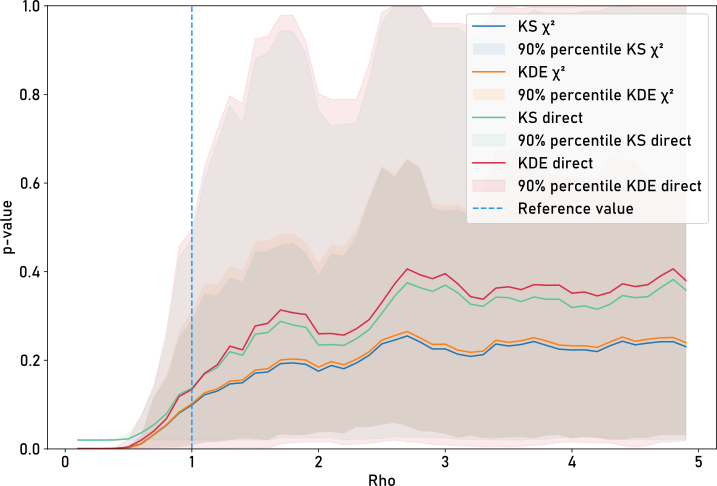
\includegraphics[width=0.49\textwidth]{figures/neutrality_test/gc_2_rho.pdf}
    \caption[Robustness of the neutrality test for $\kappa = 2$ as reference.]{Robustness of the neutrality test for different $\theta$ (left), $\rho$ (right) values
        with $\kappa = 2$ as reference.}
    \label{app:robust_gc}
\end{figure}
\newpage
\section{Runtime}\label{app:runtime}
The first differences of the recorded runtime of \mintinline{python}{gene_model} for different parameters and the absolute runtime for different $\theta / \rho$ ratios are presented here.

\begin{figure}[H]
    \centering
    \includegraphics[width=0.6\textwidth]{figures/runtime/theta_rho_heat.pdf}
    \caption[Runtime of $\theta / \rho$ ratios.]{Runtime of \mintinline{python}{gene_model} for different $\theta / \rho$ ratios for 10 samples and $\kappa = \gamma = 0$.}
    \label{app:theta-rho-heatmap}
\end{figure}
\begin{figure}[H]
    \begin{flushright}
        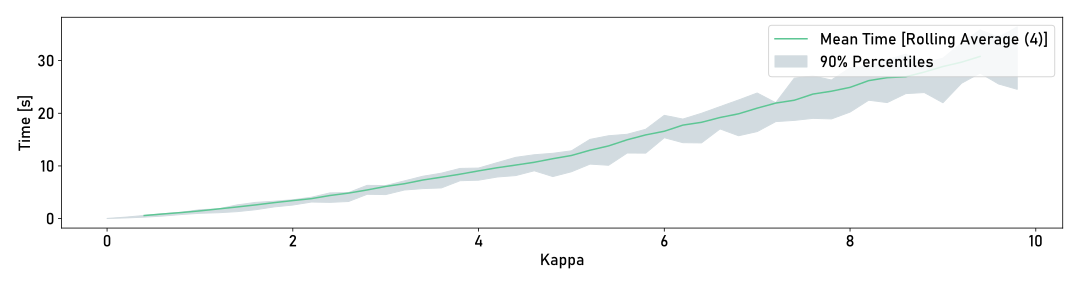
\includegraphics[width=0.988\textwidth]{figures/runtime/gene_conversion_rate_large.pdf}
    \end{flushright}
    \centering
    \caption[Runtime without HGT.]{Runtime of \mintinline{python}{gene_model} for different $\kappa$ rates for simulations without HGT.}
    \label{app:runtime-ext}
\end{figure}

\begin{figure}[H]
    \begin{flushright}
        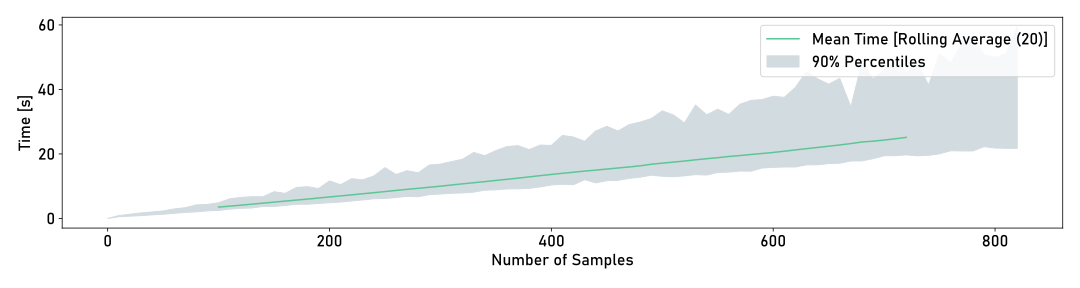
\includegraphics[width=0.995\textwidth]{figures/runtime/hgt_num_samples.pdf}\\
        \includegraphics[width=\textwidth]{figures/runtime/hgt_num_sites.pdf}\\
        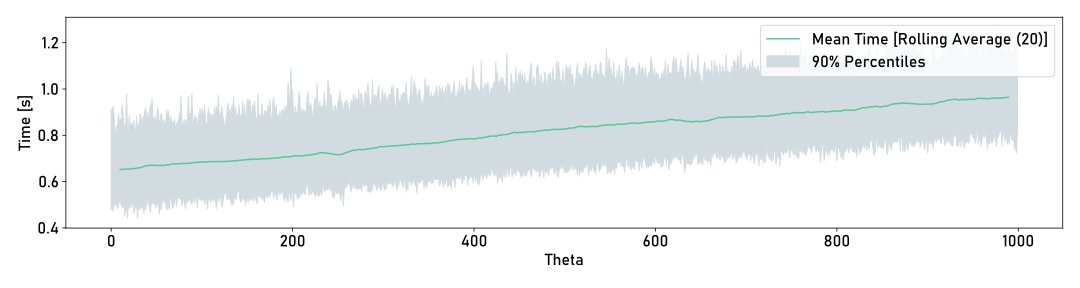
\includegraphics[width=\textwidth]{figures/runtime/hgt_theta.pdf}\\
        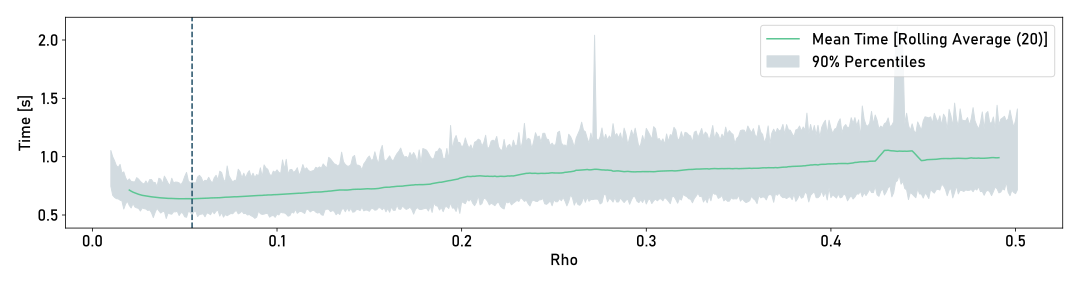
\includegraphics[width=\textwidth]{figures/runtime/hgt_rho.pdf}\\
        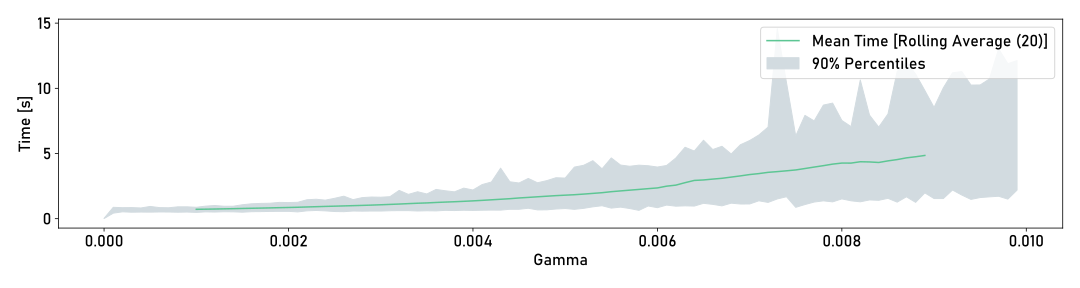
\includegraphics[width=0.995\textwidth]{figures/runtime/hgt_hgt_rate.pdf}
    \end{flushright}
    \centering
    \caption[Runtime with HGT.]{Runtime of \mintinline{python}{gene_model} for different number of samples, number of sites, $\theta$, $\rho$ and $\gamma$ rates
        for simulations with HGT.}
    \label{app:runtime-hgt}
\end{figure}
\begin{figure}[H]
    \begin{flushright}
        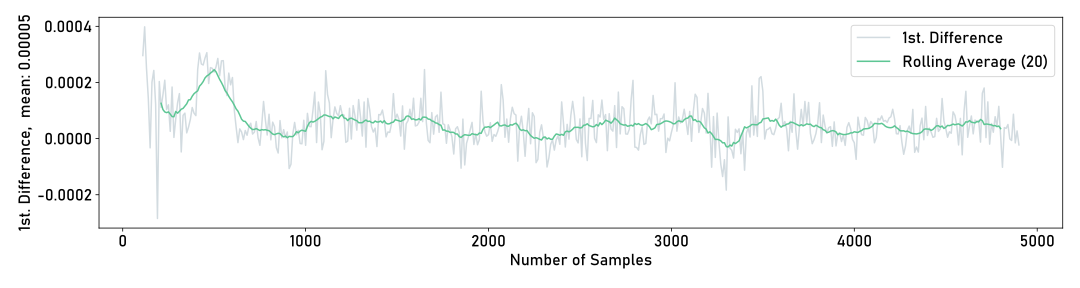
\includegraphics[width=\textwidth]{figures/runtime/num_samples_diff.pdf}\\
        \includegraphics[width=\textwidth]{figures/runtime/num_sites_diff.pdf}\\
        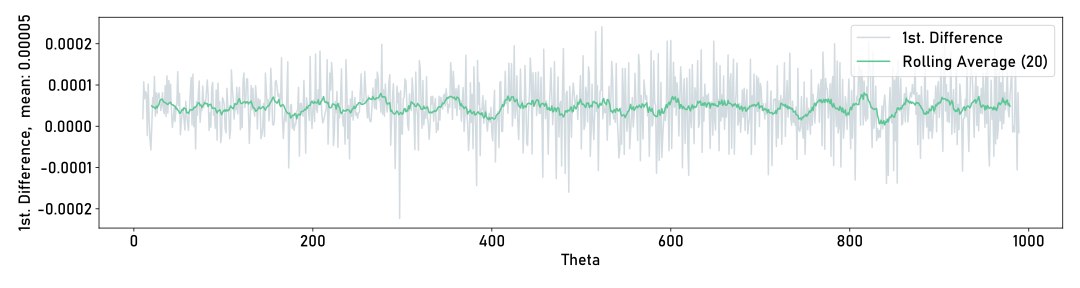
\includegraphics[width=\textwidth]{figures/runtime/theta_diff.pdf}\\
        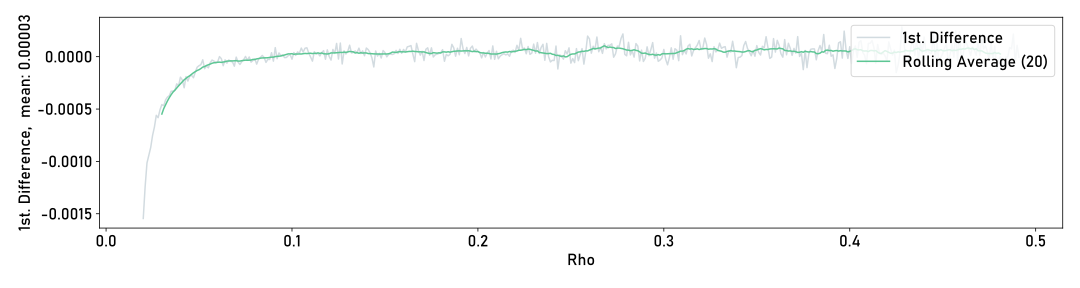
\includegraphics[width=\textwidth]{figures/runtime/rho_diff.pdf}\\
        \includegraphics[width=0.975\textwidth]{figures/runtime/gene_conversion_rate_large_diff.pdf}
    \end{flushright}
    \centering
    \caption[First difference of runtime without HGT.]{First difference of runtime of \mintinline{python}{gene_model} for different number of samples, number of sites, $\theta$, $\rho$ and $\kappa$ rates
        for simulations without HGT.}
    \label{app:diff-runtime}
\end{figure}

\begin{figure}[H]
    \begin{flushright}
        \includegraphics[width=0.983\textwidth]{figures/runtime/hgt_num_samples_diff.pdf}\\
        \includegraphics[width=0.992\textwidth]{figures/runtime/hgt_num_sites_diff.pdf}\\
        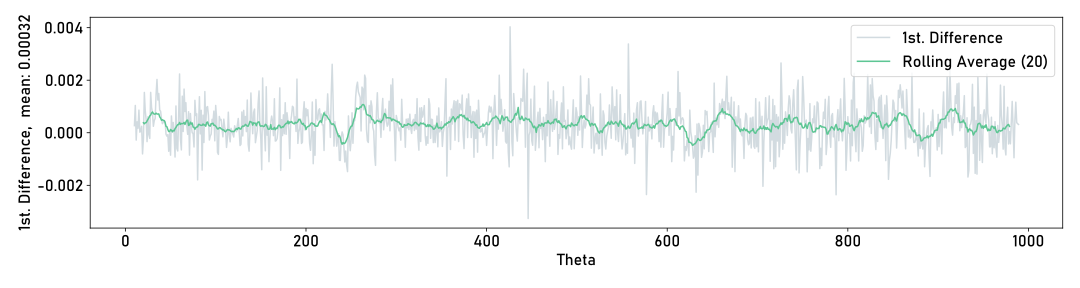
\includegraphics[width=\textwidth]{figures/runtime/hgt_theta_diff.pdf}\\
        \includegraphics[width=0.988\textwidth]{figures/runtime/hgt_rho_diff.pdf}\\
        \includegraphics[width=0.988\textwidth]{figures/runtime/hgt_hgt_rate_diff.pdf}
    \end{flushright}
    \centering
    \caption[First difference of runtime with HGT.]{First difference of runtime of \mintinline{python}{gene_model} for different number of samples, number of sites, $\theta$, $\rho$ and $\gamma$ rates
        for simulations with HGT.}
    \label{app:diff-runtime-hgt}
\end{figure}
\section{Trees for parameter estimation}
\begin{figure}[H]
    \begin{flushleft}
        \includegraphics[width=0.49\textwidth]{figures/panX_trees/803.pdf}
        \includegraphics[width=0.49\textwidth]{figures/panX_trees/985002.pdf}\\
        \includegraphics[width=0.49\textwidth]{figures/panX_trees/1492.pdf}\\
        \includegraphics[width=\textwidth]{figures/panX_trees/9.pdf}
    \end{flushleft}
    \centering
    \caption[Trees for parameter estimation.]{Phylogenetic trees inferred by \textit{PanX} and used for parameter estimation.
        From top to bottom: Bartonella quintana, Staphylococcus argenteus, Clostridium butyricum and Buchnera aphidicola.}
    \label{app:panX-trees}
\end{figure}

\section{Software and Package Versions}
\begin{table}[H]
    %\begin{adjustbox}{width=\textwidth}
    \begin{tabular}{l|l|l}
        Name                 & Version & Reference                                                                                    \\
        \hline
        bintrees             & 2.2.0   & \href{https://pypi.org/project/bintrees/}{pypi.org/project/bintrees}                         \\
        matplotlib           & 3.8.0   & \href{https://matplotlib.org/}{matplotlib.org}                                               \\
        msprime              & 1.3.1   & \href{https://tskit.dev/software/msprime.html}{tskit.dev/software/msprime.html}              \\
        numpy                & 1.26.4  & \href{https://numpy.org/}{numpy.org/}                                                        \\
        pandas               & 2.2.0   & \href{https://pandas.pydata.org/}{pandas.pydata.org}                                         \\
        python               & 3.12.1  & \href{https://www.python.org/}{python.org}                                                   \\
        scipy                & 1.12.0  & \href{https://scipy.org/}{scipy.org}                                                         \\
        seaborn              & 0.12.2  & \href{https://seaborn.pydata.org/}{seaborn.pydata.org}                                       \\
        statsmodels          & 0.14.1  & \href{https://www.statsmodels.org/stable/index.html}{statsmodels.org/stable}                 \\
        tskit                & 0.5.6   & \href{https://tskit.dev/software/tskit.html}{tskit.dev/software/tskit.html}                  \\
        tskit-arg-visualizer & 0.0.1   & \href{https://pypi.org/project/tskit-arg-visualizer/}{pypi.org/project/tskit-arg-visualizer}
    \end{tabular}
    %\end{adjustbox}
    \label{app:package-versions}
\end{table}
An installable conda environment is available on GitHub:\\
\href{https://github.com/not-a-feature/pangenome-gene-transfer-simulation/blob/main/conda_env.yml}{pangenome-gene-transfer-simulation/blob/main/conda\_env.yml}.

\section{Sustainability}
Most of the simulations were run on an Intel \textsuperscript{\textregistered} Core \texttrademark ~i5-13500 processor with a peak power consumption of 154W.
Taking into account additional overheads for cooling, idle GPU and other components, the estimated total power consumption is 200W.
The remaining simulations were run on an AMD Ryzen \texttrademark ~Threadripper \texttrademark ~3970X 32-core processor with a peak power consumption of 280W.
This would give an approximate total power consumption of 350W.
Total test and simulation durations were estimated at 350 and 50 hours respectively.

The resulting energy consumption was 87.5 kWh, supplied by a 100\% renewable energy supplier.

%%%%%%%%%%%%%%%%%%%%%%%%%%%%%%%%%%%%%%%%%%%%%%%%%%%%%%%%%%%%%%%%%%%%%%%%%%%%%
%%% Bibliographie
%%%%%%%%%%%%%%%%%%%%%%%%%%%%%%%%%%%%%%%%%%%%%%%%%%%%%%%%%%%%%%%%%%%%%%%%%%%%%

\addcontentsline{toc}{chapter}{Bibliography}
\setlength\bibitemsep{\baselineskip}
%\newgeometry{top=25mm, left=30mm, right=30mm, bottom=30mm}
\printbibliography[]

\newpage
%\cleardoublepage

%%%%%%%%%%%%%%%%%%%%%%%%%%%%%%%%%%%%%%%%%%%%%%%%%%%%%%%%%%%%%%%%%%%%%%%%%%%%%
%%% Erklaerung
%%%%%%%%%%%%%%%%%%%%%%%%%%%%%%%%%%%%%%%%%%%%%%%%%%%%%%%%%%%%%%%%%%%%%%%%%%%%%
\addcontentsline{toc}{chapter}{Selbstständigkeitserklärung}
\thispagestyle{empty}
\section*{Selbständigkeitserklärung}

Hiermit versichere ich, dass ich die vorliegende Masterarbeit selbständig und
nur mit den angegebenen Hilfsmitteln angefertigt habe und dass alle Stellen,
die dem Wortlaut oder dem Sinne nach anderen Werken entnommen sind, durch
Angaben von Quellen als Entlehnung kenntlich gemacht worden sind.
Diese Masterarbeit wurde in gleicher oder ähnlicher Form in keinem anderen
Studiengang als Prüfungsleistung vorgelegt.


\vskip 3cm
\textbf{Ort, Datum}	\hfill \textbf{Unterschrift} \hfill
\pagestyle{empty}
\cleardoublepage
\end{document}

